
%% bare_jrnl.tex
%% V1.4b
%% 2015/08/26
%% by Michael Shell
%% see http://www.michaelshell.org/
%% for current contact information.
%%
%% This is a skeleton file demonstrating the use of IEEEtran.cls
%% (requires IEEEtran.cls version 1.8b or later) with an IEEE
%% journal paper.
%%
%% Support sites:
%% http://www.michaelshell.org/tex/ieeetran/
%% http://www.ctan.org/pkg/ieeetran
%% and
%% http://www.ieee.org/

%%*************************************************************************
%% Legal Notice:
%% This code is offered as-is without any warranty either expressed or
%% implied; without even the implied warranty of MERCHANTABILITY or
%% FITNESS FOR A PARTICULAR PURPOSE! 
%% User assumes all risk.
%% In no event shall the IEEE or any contributor to this code be liable for
%% any damages or losses, including, but not limited to, incidental,
%% consequential, or any other damages, resulting from the use or misuse
%% of any information contained here.
%%
%% All comments are the opinions of their respective authors and are not
%% necessarily endorsed by the IEEE.
%%
%% This work is distributed under the LaTeX Project Public License (LPPL)
%% ( http://www.latex-project.org/ ) version 1.3, and may be freely used,
%% distributed and modified. A copy of the LPPL, version 1.3, is included
%% in the base LaTeX documentation of all distributions of LaTeX released
%% 2003/12/01 or later.
%% Retain all contribution notices and credits.
%% ** Modified files should be clearly indicated as such, including  **
%% ** renaming them and changing author support contact information. **
%%*************************************************************************


% *** Authors should verify (and, if needed, correct) their LaTeX system  ***
% *** with the testflow diagnostic prior to trusting their LaTeX platform ***
% *** with production work. The IEEE's font choices and paper sizes can   ***
% *** trigger bugs that do not appear when using other class files.       ***                          ***
% The testflow support page is at:
% http://www.michaelshell.org/tex/testflow/



\documentclass[journal]{IEEEtran}
%
% If IEEEtran.cls has not been installed into the LaTeX system files,
% manually specify the path to it like:
% \documentclass[journal]{../sty/IEEEtran}


% Some very useful LaTeX packages include:
% (uncomment the ones you want to load)


% *** MISC UTILITY PACKAGES ***
%
%\usepackage{ifpdf}
% Heiko Oberdiek's ifpdf.sty is very useful if you need conditional
% compilation based on whether the output is pdf or dvi.
% usage:
% \ifpdf
%   % pdf code
% \else
%   % dvi code
% \fi
% The latest version of ifpdf.sty can be obtained from:
% http://www.ctan.org/pkg/ifpdf
% Also, note that IEEEtran.cls V1.7 and later provides a builtin
% \ifCLASSINFOpdf conditional that works the same way.
% When switching from latex to pdflatex and vice-versa, the compiler may
% have to be run twice to clear warning/error messages.


% *** CITATION PACKAGES ***
%
%\usepackage{cite}
% cite.sty was written by Donald Arseneau
% V1.6 and later of IEEEtran pre-defines the format of the cite.sty package
% \cite{} output to follow that of the IEEE. Loading the cite package will
% result in citation numbers being automatically sorted and properly
% "compressed/ranged". e.g., [1], [9], [2], [7], [5], [6] without using
% cite.sty will become [1], [2], [5]--[7], [9] using cite.sty. cite.sty's
% \cite will automatically add leading space, if needed. Use cite.sty's
% noadjust option (cite.sty V3.8 and later) if you want to turn this off
% such as if a citation ever needs to be enclosed in parenthesis.
% cite.sty is already installed on most LaTeX systems. Be sure and use
% version 5.0 (2009-03-20) and later if using hyperref.sty.
% The latest version can be obtained at:
% http://www.ctan.org/pkg/cite
% The documentation is contained in the cite.sty file itself.


% *** GRAPHICS RELATED PACKAGES ***
%
\ifCLASSINFOpdf
  % \usepackage[pdftex]{graphicx}
  % declare the path(s) where your graphic files are
  % \graphicspath{{../pdf/}{../jpeg/}}
  % and their extensions so you won't have to specify these with
  % every instance of \includegraphics
  % \DeclareGraphicsExtensions{.pdf,.jpeg,.png}
\else
  % or other class option (dvipsone, dvipdf, if not using dvips). graphicx
  % will default to the driver specified in the system graphics.cfg if no
  % driver is specified.
  % \usepackage[dvips]{graphicx}
  % declare the path(s) where your graphic files are
  % \graphicspath{{../eps/}}
  % and their extensions so you won't have to specify these with
  % every instance of \includegraphics
  % \DeclareGraphicsExtensions{.eps}
\fi
% graphicx was written by David Carlisle and Sebastian Rahtz. It is
% required if you want graphics, photos, etc. graphicx.sty is already
% installed on most LaTeX systems. The latest version and documentation
% can be obtained at: 
% http://www.ctan.org/pkg/graphicx
% Another good source of documentation is "Using Imported Graphics in
% LaTeX2e" by Keith Reckdahl which can be found at:
% http://www.ctan.org/pkg/epslatex
%
% latex, and pdflatex in dvi mode, support graphics in encapsulated
% postscript (.eps) format. pdflatex in pdf mode supports graphics
% in .pdf, .jpeg, .png and .mps (metapost) formats. Users should ensure
% that all non-photo figures use a vector format (.eps, .pdf, .mps) and
% not a bitmapped formats (.jpeg, .png). The IEEE frowns on bitmapped formats
% which can result in "jaggedy"/blurry rendering of lines and letters as
% well as large increases in file sizes.
%
% You can find documentation about the pdfTeX application at:
% http://www.tug.org/applications/pdftex


% *** MATH PACKAGES ***
%
%\usepackage{amsmath}
% A popular package from the American Mathematical Society that provides
% many useful and powerful commands for dealing with mathematics.
%
% Note that the amsmath package sets \interdisplaylinepenalty to 10000
% thus preventing page breaks from occurring within multiline equations. Use:
%\interdisplaylinepenalty=2500
% after loading amsmath to restore such page breaks as IEEEtran.cls normally
% does. amsmath.sty is already installed on most LaTeX systems. The latest
% version and documentation can be obtained at:
% http://www.ctan.org/pkg/amsmath


% *** SPECIALIZED LIST PACKAGES ***
%
%\usepackage{algorithmic}
% algorithmic.sty was written by Peter Williams and Rogerio Brito.
% This package provides an algorithmic environment fo describing algorithms.
% You can use the algorithmic environment in-text or within a figure
% environment to provide for a floating algorithm. Do NOT use the algorithm
% floating environment provided by algorithm.sty (by the same authors) or
% algorithm2e.sty (by Christophe Fiorio) as the IEEE does not use dedicated
% algorithm float types and packages that provide these will not provide
% correct IEEE style captions. The latest version and documentation of
% algorithmic.sty can be obtained at:
% http://www.ctan.org/pkg/algorithms
% Also of interest may be the (relatively newer and more customizable)
% algorithmicx.sty package by Szasz Janos:
% http://www.ctan.org/pkg/algorithmicx


% *** ALIGNMENT PACKAGES ***
%
%\usepackage{array}
% Frank Mittelbach's and David Carlisle's array.sty patches and improves
% the standard LaTeX2e array and tabular environments to provide better
% appearance and additional user controls. As the default LaTeX2e table
% generation code is lacking to the point of almost being broken with
% respect to the quality of the end results, all users are strongly
% advised to use an enhanced (at the very least that provided by array.sty)
% set of table tools. array.sty is already installed on most systems. The
% latest version and documentation can be obtained at:
% http://www.ctan.org/pkg/array


% IEEEtran contains the IEEEeqnarray family of commands that can be used to
% generate multiline equations as well as matrices, tables, etc., of high
% quality.


% *** SUBFIGURE PACKAGES ***
%\ifCLASSOPTIONcompsoc
%  \usepackage[caption=false,font=normalsize,labelfont=sf,textfont=sf]{subfig}
%\else
%  \usepackage[caption=false,font=footnotesize]{subfig}
%\fi
% subfig.sty, written by Steven Douglas Cochran, is the modern replacement
% for subfigure.sty, the latter of which is no longer maintained and is
% incompatible with some LaTeX packages including fixltx2e. However,
% subfig.sty requires and automatically loads Axel Sommerfeldt's caption.sty
% which will override IEEEtran.cls' handling of captions and this will result
% in non-IEEE style figure/table captions. To prevent this problem, be sure
% and invoke subfig.sty's "caption=false" package option (available since
% subfig.sty version 1.3, 2005/06/28) as this is will preserve IEEEtran.cls
% handling of captions.
% Note that the Computer Society format requires a larger sans serif font
% than the serif footnote size font used in traditional IEEE formatting
% and thus the need to invoke different subfig.sty package options depending
% on whether compsoc mode has been enabled.
%
% The latest version and documentation of subfig.sty can be obtained at:
% http://www.ctan.org/pkg/subfig


% *** FLOAT PACKAGES ***
%
%\usepackage{fixltx2e}
% fixltx2e, the successor to the earlier fix2col.sty, was written by
% Frank Mittelbach and David Carlisle. This package corrects a few problems
% in the LaTeX2e kernel, the most notable of which is that in current
% LaTeX2e releases, the ordering of single and double column floats is not
% guaranteed to be preserved. Thus, an unpatched LaTeX2e can allow a
% single column figure to be placed prior to an earlier double column
% figure.
% Be aware that LaTeX2e kernels dated 2015 and later have fixltx2e.sty's
% corrections already built into the system in which case a warning will
% be issued if an attempt is made to load fixltx2e.sty as it is no longer
% needed.
% The latest version and documentation can be found at:
% http://www.ctan.org/pkg/fixltx2e


%\usepackage{stfloats}
% stfloats.sty was written by Sigitas Tolusis. This package gives LaTeX2e
% the ability to do double column floats at the bottom of the page as well
% as the top. (e.g., "\begin{figure*}[!b]" is not normally possible in
% LaTeX2e). It also provides a command:
%\fnbelowfloat
% to enable the placement of footnotes below bottom floats (the standard
% LaTeX2e kernel puts them above bottom floats). This is an invasive package
% which rewrites many portions of the LaTeX2e float routines. It may not work
% with other packages that modify the LaTeX2e float routines. The latest
% version and documentation can be obtained at:
% http://www.ctan.org/pkg/stfloats
% Do not use the stfloats baselinefloat ability as the IEEE does not allow
% \baselineskip to stretch. Authors submitting work to the IEEE should note
% that the IEEE rarely uses double column equations and that authors should try
% to avoid such use. Do not be tempted to use the cuted.sty or midfloat.sty
% packages (also by Sigitas Tolusis) as the IEEE does not format its papers in
% such ways.
% Do not attempt to use stfloats with fixltx2e as they are incompatible.
% Instead, use Morten Hogholm'a dblfloatfix which combines the features
% of both fixltx2e and stfloats:
%
% \usepackage{dblfloatfix}
% The latest version can be found at:
% http://www.ctan.org/pkg/dblfloatfix


%\ifCLASSOPTIONcaptionsoff
%  \usepackage[nomarkers]{endfloat}
% \let\MYoriglatexcaption\caption
% \renewcommand{\caption}[2][\relax]{\MYoriglatexcaption[#2]{#2}}
%\fi
% endfloat.sty was written by James Darrell McCauley, Jeff Goldberg and 
% Axel Sommerfeldt. This package may be useful when used in conjunction with 
% IEEEtran.cls'  captionsoff option. Some IEEE journals/societies require that
% submissions have lists of figures/tables at the end of the paper and that
% figures/tables without any captions are placed on a page by themselves at
% the end of the document. If needed, the draftcls IEEEtran class option or
% \CLASSINPUTbaselinestretch interface can be used to increase the line
% spacing as well. Be sure and use the nomarkers option of endfloat to
% prevent endfloat from "marking" where the figures would have been placed
% in the text. The two hack lines of code above are a slight modification of
% that suggested by in the endfloat docs (section 8.4.1) to ensure that
% the full captions always appear in the list of figures/tables - even if
% the user used the short optional argument of \caption[]{}.
% IEEE papers do not typically make use of \caption[]'s optional argument,
% so this should not be an issue. A similar trick can be used to disable
% captions of packages such as subfig.sty that lack options to turn off
% the subcaptions:
% For subfig.sty:
% \let\MYorigsubfloat\subfloat
% \renewcommand{\subfloat}[2][\relax]{\MYorigsubfloat[]{#2}}
% However, the above trick will not work if both optional arguments of
% the \subfloat command are used. Furthermore, there needs to be a
% description of each subfigure *somewhere* and endfloat does not add
% subfigure captions to its list of figures. Thus, the best approach is to
% avoid the use of subfigure captions (many IEEE journals avoid them anyway)
% and instead reference/explain all the subfigures within the main caption.
% The latest version of endfloat.sty and its documentation can obtained at:
% http://www.ctan.org/pkg/endfloat
%
% The IEEEtran \ifCLASSOPTIONcaptionsoff conditional can also be used
% later in the document, say, to conditionally put the References on a 
% page by themselves.


% *** PDF, URL AND HYPERLINK PACKAGES ***
%
%\usepackage{url}
% url.sty was written by Donald Arseneau. It provides better support for
% handling and breaking URLs. url.sty is already installed on most LaTeX
% systems. The latest version and documentation can be obtained at:
% http://www.ctan.org/pkg/url
% Basically, \url{my_url_here}.


% *** Do not adjust lengths that control margins, column widths, etc. ***
% *** Do not use packages that alter fonts (such as pslatex).         ***
% There should be no need to do such things with IEEEtran.cls V1.6 and later.
% (Unless specifically asked to do so by the journal or conference you plan
% to submit to, of course. )

\usepackage{graphics} % for pdf, bitmapped graphics files
\usepackage{epsfig} % for postscript graphics files
\usepackage{mathptmx} % assumes new font selection scheme installed
\usepackage{times} % assumes new font selection scheme installed
\usepackage{amsmath} % assumes amsmath package installed
\usepackage{amssymb}  % assumes amsmath package installed
%\usepackage{amsthm}
\usepackage{bm}
\usepackage{mathrsfs}
\usepackage{xcolor}
\usepackage{cite}
\usepackage{threeparttable}
\usepackage{multirow}
\usepackage{bigdelim}
\usepackage{algorithm}
\usepackage{algorithmicx}
\usepackage{algpseudocode}
\usepackage{graphicx}
\usepackage{subfigure}
\usepackage{comment}

% correct bad hyphenation here
\hyphenation{op-tical net-works semi-conduc-tor}


\begin{document}
%
% paper title
% Titles are generally capitalized except for words such as a, an, and, as,
% at, but, by, for, in, nor, of, on, or, the, to and up, which are usually
% not capitalized unless they are the first or last word of the title.
% Linebreaks \\ can be used within to get better formatting as desired.
% Do not put math or special symbols in the title.
\title{Cellular Decomposition for Non-repetitive Coverage Task Ensuring Least Discontinuities}
%
%
% author names and IEEE memberships
% note positions of commas and nonbreaking spaces ( ~ ) LaTeX will not break
% a structure at a ~ so this keeps an author's name from being broken across
% two lines.
% use \thanks{} to gain access to the first footnote area
% a separate \thanks must be used for each paragraph as LaTeX2e's \thanks
% was not built to handle multiple paragraphs
%

%\author{Michael~Shell,~\IEEEmembership{Member,~IEEE,}
%        John~Doe,~\IEEEmembership{Fellow,~OSA,}
%        and~Jane~Doe,~\IEEEmembership{Life~Fellow,~IEEE}% <-this % stops a space
%\thanks{M. Shell was with the Department
%of Electrical and Computer Engineering, Georgia Institute of Technology, Atlanta,
%GA, 30332 USA e-mail: (see http://www.michaelshell.org/contact.html).}% <-this % stops a space
%\thanks{J. Doe and J. Doe are with Anonymous University.}% <-this % stops a space
%\thanks{Manuscript received April 19, 2005; revised August 26, 2015.}}

\author{Tong Yang$^1$, Jaime Valls Miro$^2$, Qianen Lai$^1$, Yue Wang$^{1*}$ and Rong Xiong$^1$
\thanks{$^1$ Tong Yang, Qianen Lai, Yue Wang and Rong Xiong are with the State Key Laboratory of Industrial Control and Technology, Zhejiang University, P.R. China. 
%Yue Wang is the corresponding author {\tt\small wangyue@iipc.zju.edu.cn}. Rong Xiong is the co-corresponding author {\tt\small rxiong@zju.edu.cn}.
}
\thanks{$^2$ Jaime Valls Miro is with the Centre for Autonomous Systems (CAS), Faculty of Engineering, University of Technology Sydney (UTS), NSW 2007 Sydney, Australia.}
\thanks{$^*$ Corresponding Author. \newline \indent
E-mail address: {\tt\small wangyue@iipc.zju.edu.cn}}
}

% note the % following the last \IEEEmembership and also \thanks - 
% these prevent an unwanted space from occurring between the last author name
% and the end of the author line. i.e., if you had this:
% 
% \author{....lastname \thanks{...} \thanks{...} }
%                     ^------------^------------^----Do not want these spaces!
%
% a space would be appended to the last name and could cause every name on that
% line to be shifted left slightly. This is one of those "LaTeX things". For
% instance, "\textbf{A} \textbf{B}" will typeset as "A B" not "AB". To get
% "AB" then you have to do: "\textbf{A}\textbf{B}"
% \thanks is no different in this regard, so shield the last } of each \thanks
% that ends a line with a % and do not let a space in before the next \thanks.
% Spaces after \IEEEmembership other than the last one are OK (and needed) as
% you are supposed to have spaces between the names. For what it is worth,
% this is a minor point as most people would not even notice if the said evil
% space somehow managed to creep in.


% The paper headers
\markboth{This paper is concurrently submitted for TMech and AIM 2020 Presentation}{}
%\markboth{Journal of \LaTeX\ Class Files,~Vol.~14, No.~8, August~2015}%
%{Tong \MakeLowercase{\textit{et al.}}: Cellular Decomposition for Non-repetitive Coverage Task Ensuring Least Discontinuities}
% The only time the second header will appear is for the odd numbered pages
% after the title page when using the twoside option.
% 
% *** Note that you probably will NOT want to include the author's ***
% *** name in the headers of peer review papers.                   ***
% You can use \ifCLASSOPTIONpeerreview for conditional compilation here if
% you desire.


% If you want to put a publisher's ID mark on the page you can do it like
% this:
%\IEEEpubid{0000--0000/00\$00.00~\copyright~2015 IEEE}
% Remember, if you use this you must call \IEEEpubidadjcol in the second
% column for its text to clear the IEEEpubid mark.

% use for special paper notices
%\IEEEspecialpapernotice{(Invited Paper)}


% make the title area
\maketitle

% As a general rule, do not put math, special symbols or citations
% in the abstract or keywords.
\begin{abstract}
% <jvm> needs to be shorten and sharpened substantially ... TO BE LEFT FOR last, leave for now
There are many non-repetitive coverage tasks which use a high-dimensional path to cover low-dimensional space, such as the polishing task using the manipulators. Due to the non-bijective mapping between the workspace and the joint-space, a continuous coverage path in the workspace is truncated in the joint-space, and there are multiple choices of configurations to cover a same waypoint of the coverage path. 
The discontinuous point implies a suspension of the coverage task, which is difficult to handle. For example. the suspension of the polishing task means the lift-off the end-effector from the surface of the object, where the transition between the force/position control is required, which is more complicated than the ordinary coverage process. 

In this paper, motivated by the non-repetitive coverage task of non-redundant manipulators, we first prove that the least number of discontinuity is a parameter of the environment setting, independent to the choice of coverage paths, thus has a minimum. 
Then, a cellular decomposition method generating all optimal cellular decompositions is proposed. 
The algorithm is operational in any dimension, and we illustrate it through polishing tasks.
Through simulated experiments, the least number of discontinuities is shown as a novel criterion of the quality of the placement of the manipulator (or the object). Besides, the method helps to solve the problem of multiple inverse kinematic (IK) solutions. In real-world experiment, the physical coverage path is generated to show the applicability of the proposed algorithm. \textcolor{blue}{The video of the real-world experiments is given here: }.
\end{abstract}

% Note that keywords are not normally used for peerreview papers.
%\begin{IEEEkeywords}
%cellular decomposition, coverage task, non-redundant manipulator
%\end{IEEEkeywords}


% For peer review papers, you can put extra information on the cover
% page as needed:
% \ifCLASSOPTIONpeerreview
% \begin{center} \bfseries EDICS Category: 3-BBND \end{center}
% \fi
%
% For peerreview papers, this IEEEtran command inserts a page break and
% creates the second title. It will be ignored for other modes.
\IEEEpeerreviewmaketitle

\section{Introduction}
% The very first letter is a 2 line initial drop letter followed
% by the rest of the first word in caps.
% 
% form to use if the first word consists of a single letter:
% \IEEEPARstart{A}{demo} file is ....
% 
% form to use if you need the single drop letter followed by
% normal text (unknown if ever used by the IEEE):
% \IEEEPARstart{A}{}demo file is ....
% 
% Some journals put the first two words in caps:
% \IEEEPARstart{T}{his demo} file is ....
% 
% Here we have the typical use of a "T" for an initial drop letter
% and "HIS" in caps to complete the first word.
\IEEEPARstart{T}{he} non-repetitive \textit{coverage task} of a given object is an important application carried out by manipulators.
This is for instance the case of inspecting a surface for defects at close range, painting, deburring or polishing. 
The task is effectively encapsulated as the generic coverage path planning (CPP)~\cite{choset2001coverage}~\cite{galceran2013a} problem, which requires for the end-effector (EE) to traverse over all the points that define the surface of a given object exactly one time, whilst usually 
fulfilling additional task-specific constraints (e.g.  sustain a desired orientation of the EE with respect to the surface, maintain contact or exerting a constant EE force/torque). 
Typically, joint-space dimension is higher than the workspace's, % such as using a non-redundant manipulator to polish a surface, 
and the inverse kinematic (IK) mapping between task and joint space is thus non-bijective.  
%(unique one-to-one correspondences between input-output domains can not be established). 
%Fixed <jvm> I believe this is always the case and we can say so this way  - Tong pls share your view responding to this comment 
% <ty> Yes, the problem of multiple solutions always exists for the revolute joint, and the usage of "non-bijective" is always valid. 
% Yue Wang thought "bijective" is not appropriate, since the mapping is not valid on the whole task-space and the joint-space, but we didn't find a word to express it. Now that you restrict "input-output domains", then both "bijective" and "non-bijective" make sense. 
As a result, planning in the higher dimension joint-space cannot ensure non-repetitive visiting, 
\begin{color}{blue}
with the task-to-joint mapping being non-injective, 
\end{color}
and coverage paths are thus more suited to be designed directly in the workspace domain~\cite{Oriolo2005Motion}.  
% <ty> (1) Are the above two sentences repeated? so we can omit "with the task-to-joint mapping being non-injective"
%      (2) if the sentence is necessary for detailed explanation, then "task-to-joint" should be "joint-to-task". 

\begin{figure}[t]
\centering
\subfigure[Relationship between joint- and work-space.]{
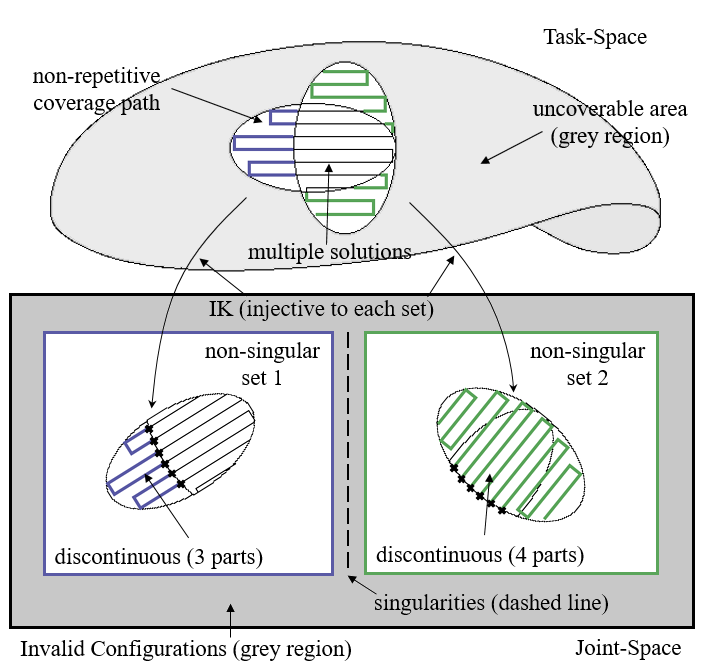
\includegraphics[width = 0.4\textwidth]{fig1_mark_singular}
}
\subfigure[Greedy solution example]{
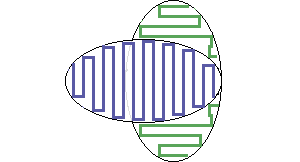
\includegraphics[width = 0.22\textwidth]{greedy}
\label{fig:greedy}
}
\subfigure[Optimal solution example]{
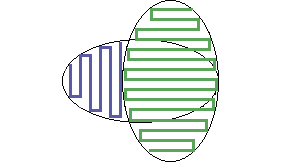
\includegraphics[width = 0.22\textwidth]{optimal}
\label{fig:optimal}
}
\caption{(a) Illustration of the coverage task problem and the relationship between joint- and work-space. 
Different colors denote disjoint sets of non-singular 
%multi-dimensional 
joint configurations (arbitrarily, blue may for instance represent those with 
elbow-up, whilst green may represent elbow-down), and their corresponding path in the workspace. 
The colored segments of the arbitrary coverage path shown in black have unique IK solutions. However, multiple IK solutions exist for the intersecting area shown in black.
%thus requiring further planning decisions. 
The underlying continuous coverage path sought out thus becomes intermittent in the workspace after mapping onto the joint-space.
In this example, whatever choice among the multiple IK solutions, six discontinuities are required 
(depicted by black crosses), since the path has three separate segments in set $1$, and four in set $2$. 
The case where the joint-space solutions are taken in full from set 2 (green) is depicted.
(b) Starting from a configuration belonging to set $1$, without explicitly calculating the reachable boundary of each set, the boundary of the set $2$ within the reachable area of set $1$ is unknown. So a greedy strategy will fully cover the set $1$, dividing the uncovered region into two parts, leading to an extra lift-off. 
On the other hand, although at first sight it may appear the same as using the greedy strategy starting from set $2$ (c) illustrates the concept of CPP optimality' in the joint space, whereby the continuity of the reachable area is explicitly considered, thus producing a coverage path with a single EE lift-off.} 
%Fixed <jvm> Tong pls change pic to reflect this, with lift-off crosses on inside semi-circle in set 1, and as they are in set 2
% <ty> I understood your idea, and I hope the newly added figures showing an optimal solution and a non-optimal greedy solution help to explain the problem without words (to save the pages).
\label{fig1}
\end{figure}

Yet what constitutes a continuous coverage path in the workspace may easily end up truncated into many seemingly \textit{intermittent} sections after mapping them back onto the joint-space, with undersirable path discontinuities, as graphically illustrated by Fig.~\ref{fig1}. 
This is also the case if a simplistic greedy strategy is followed, as the example depicted in Fig.~\ref{fig:greedy}, whereby a complete path in task space that solves for all possible configurations leads to unnecessary lift-offs to accomplish full coverage. 
The problem is further compounded by additional task constraints, most notably obstacles, which produce usable configurations further divided into many disjoint sets, possibily requiring more undesirable``jumps'' between sets for successful coverage. 
This work advocates for the minimisation of the cost incurred on these path discontinuities, which can significantly outweigh
any improvements that may occur locally in the task space when it comes to coverage \cite{hassan2018a}. %Fixed <jvm> ~\cite Mahdi's paper? % <ty> added
This is perhaps more apparent for the case of the uniform polishing task motivating this work, as that means lifting the EE off the object's surface, adjusting the pose of the manipulator to the new configuration, and landing back into contact with the surface again.
This may be not only sub-optimal for the speedy completion of the CPP task, but also introduces potentially avoidable complexity in transitioning between position and force/torque control~\cite{heck2015switched}~\cite{solanes2018adaptive}~\cite{solanes2019robust} during the coverage task. 
 
In this work, a mechanism is proposed to address this shortcoming and derive CPP solutions with a proven minimal number of discontinuities, with the aim to avoid unnecessary, costly EE lift-offs. 
The solution departs from locally optimising the shape of the coverage path in task space, or choosing appropiate but possibly disconnected configurations, 
but considering the reachability of each continuous motion globally.
%Fixed <jvm> this concept of "global here" is quite loose, what does it mean exactly? ... % <ty> maybe the following one
\begin{color}{blue}
The solution departs from locally optimising the shape of the coverage path in task space, or choosing appropiate but possibly disconnected configurations, 
but explicitly seeking for least number of discontinuous motion through the analysis of the structure of the valid configurations in the joint-space. 
\end{color}

%
%Fixed <jvm> I've tried to rewrite the below reasoning as it seem to lead to the contribution of the papers, where we can plan for minimal lift-off. BUT IT IS NOT CLEAR TO ME, I can't quite tell what the cause and what is the effect, it does not make much sense, or leads to the 2 ``contributions'' I then claim the paper does ... you refer to Fig 1, but in there we don't deal with singularities, is about multi IK for a given pose, so the whole idea motivating the singularity below escapes me ... am I missing something? can you pls rewrite if that's the case, and I give it another go afterwards?
% Note that the whole paragraph below could be omitted and simply leave this as motivation, without saying how we do it until later. I was looking for a succint explanation/justification of the minimumal lift-off due to the funcion being injective as you say below, but I don't see it. See further comments below.
%
% <ty> I think the causalities are follows. They are easy to show through "-->", but really difficult for me in English coherently. I hope they can answer your question:
% Our motivations are: 
%(1)    the IK is non-bijective 
%   --> planning path in joint-space cannot avoid over-visiting
%   --> use "planning-tracking" strategy, planning a path in task-space and solving IK for configurations
%   --> its disadvantage: ensuring the avoidance of over-visiting, but no guarantee of many many discontinuities
%   --> to relieve but not solve the problem, planning the path in the task-space while considering greedily choosing the configurations
%   --> we have counter-example showing the non-optimality of the greedy strategy
%   --> but the cost of an extra liftoffs is much greater than improving the coverage path (e.g. changing from boustrophedon to spiral path, as Mahdi did)
%   --> result: The problem really exists and is serious. And it is not an optimization problem of locally changing the shape of the coverage path in task-space, nor choosing more appropriate configurations. We must explicitly consider the reachability of each continuous motion, as a "global problem". 
%
% We notices that: 
%(2)    The singulities cause bifurcation, which is the ``intersections'' of different configurations (e.g. shoulder-left and shoulder-right)
%   --> disgarding all singularities, the non-singular configurations in joint-space are divided into several separated sets. In usual 5DOF or 6DOF manipulator, the physical meaning of the sets are: shoulder-left & elbow-up & wrist flipped, ... The sets look like the items shown in Fig 1. 
%   --> if we have to use two configurations which belong to different sets(here not necessarily with same pose of EE), then we must visit singularities
%   --> but the singularities are useless, so they directly imply lift-offs
%   --> with the existance of other constraints (e.g. obstacles, manipulabilities, static force constraint), even a single "set" drawn in Figure 1 may no longer be connected, implying more number of dis-joint sets, possibly requiring more number of lift-offs.
%   --> Further notice that the manipulator is omni-directional in the joint-space, so instead of considering the path, only what we need to consider is the cellular decomposition (i.e. above-mentioned "global problem" is actually a "global cellular decomposition problem".)
%   --> result: our contribution 1, and leads to our algorithm
%
% How our method does: 
%(3)    notice that the IK in each branch is injective, because there is no non-singular path connecting two configurations whose EE are at a same point(assume that it is apparent for the reviewers, since we cannot prove it through rigorous formula) 
%   --> if we assign color for all configurations based on their joint-space continuities, different IK solutions for a same pose of EE must have different colors
%   --> for a point, choosing a color means choosing a configuration, so the joint-space planning problem becomes designing a coloring scheme for the graph. 
%   --> Our concern is only the connectivity, then several equivalences make the problem (finitly) solvable. 
%   --> result: ends up with an iterative algorithm (our contribution 2)
%
The work is predicated on the fact that singularities have been proven to be the cause of bifurcation of the joint-space~\cite{porta2010path}~\cite{Porta2012Randomized}, i.e. sitting at the intersection of different configurations (e.g. elbow-up and elbow-down).
Notwithstanding singularities, for non-redundant manipulators, non-singular configurations thus form disjoint sets in the joint-space, as was illustrated by the earlier example in Fig.~\ref{fig1}. 
Moreover, due to task constraints (obstacles, joint limits, etc), commonly the whole workspace cannot be mapped into a single set, which then implies that continuous joint-space paths between sets must visit some singularities along the way, inevitably incurring undersirable lift-offs. 
However, manipulators are locally omni-directional in the joint-space, and configurations corresponding to a segment of coverage path without lift-off have high dimensional continuity in the joint-space, independently of their sequencing order. 
Hence, instead of considering the design of a coverage path in the traditional sense, this work considers the global optimal cellular decomposition problem in joint-space to incur joint-space partitions with minimum sets. 
It is further noted that IK mapping from the reachable points in the workspace to a single set of configurations is injective, since there is no non-singular path connecting two configurations whose EEs are at a same point. 
%The reason is that where different IK solutions exist, they are derived from different solutions of an inverse trigonometric function in the kinematic formulations, between which joint angles go through a singular value. %Fixed <jvm> NOTE: not sure I need to say this sentence, explains concept of singularity
% As a result, different IK solutions for a same pose belongs to different sets. %Fixed <jvm> removed as repeated?
% <ty> If the result is straightforward then these two sentences can definitely be deleted.
% This motivates the formulation of the problem of joint-space path planning effectively back into the task-space: %Fixed <jvm> I like this sentence and understand why you say, but I feel it misleads the reader to think planning is back in the workspace, it is not. Although it is injective, so effective it is ... a tad confusing ... maybe to be reused later in discussion? % <ty> Have been used in section 3. 
By assigning a class (colours are used in this paper for easier visualization) to each configuration based on their joint-space continuity, different IK solutions for a same EE pose must possess a different colour. % <ty> Here maybe the cause and the effect are inversed? The joint-space algorithm can be visualized on the surface, because we observe that the IK in each branch is injective. So I think maybe "why we use color to do visualization" is just a natual corollary of our contribution "transform the original problem into a painting problem"?  See my paragraph in section IV(C), near the end of the "third", where the words are similar to yours here.  
As such, colouring a point in the surface to be covered means selecting a given IK solution for it, 
and the planning problem is transfered to designing a colour scheme for a topological configuration graph.
In that way, the key concern is the joint-space continuity of the cells, and by efficiently discarding equivalent cellular decompositions, this work proves that total number of different cellular decompositions is finite, thus all optimal solutions are finitely solvable. 


\begin{comment}
\begin{color}{teal}
For non-redundant manipulators, non-singular configurations form disjoint sets in the joint-space, as was illustrated by the earlier example 
in Fig.~\ref{fig1}. In this work, we further note that IK mapping from the reachable points in the workspace to a single set of configurations 
is injective. % <jvm> so? can't see the link to the minimum lift-off sorry, maybe there, but in your explanation, I can't
The reason is that where different IK solutions exist, they are derived from different solutions of an inverse trigonometric function in 
the kinematic formulations, between which joint angles go through a singular value. Singularities have been proven to be the cause of 
bifurcationn of the joint-space~\cite{porta2010path}~\cite{Porta2012Randomized} % <jvm> maybe, but e.g. in Fig 1 we don't deal with singularities, and still have multiple IK solutions, which is what matters I think. I don't see the message/role about singularities that you are trying to get accross to link to the minium lift-off CPPs ....
% As a result, different IK solutions for a same pose belongs to different sets. % <jvm> removed as repeated?
Due to constraints (obstacles, joint limits, etc), commonly the whole workspace cannot be mapped into a single set, which then implies that continuous joint-space path must visit some singularities along the way, inevitably incurring lift-offs. %<jvm> again, why singularities? no singularities in Fig 1, but multi-IK solutions, none singular ...?? 
\end{color}


% <ty> I guess you want to write like this (in the tealed paragraph)
\begin{color}{blue}
From the observation in Figure \ref{fig1}, the problem cannot be relieved through (local) adjustment of the coverage path in the task-space, thus it must be solved in the joint-space. 
Besides, we notice that the configurations corresponding to a piece of coverage path without lift-off have high dimensional continuity in the joint-space~\cite{porta2010path}~\cite{Porta2012Randomized}, 
which is independent to their order. Hence, instead of considering the design of the coverage path, we can instead only consider the optimal cellular decomposition problem in the joint-space. 
Note that here the discussion is restricted in low dimension (because the manipulator is non-redundant), the algorithm for ``all valid configurations'' is computational acceptable. % <jvm> NOTE: this comment about computational tractability to be briefly added, perhaps to discussion?? here in the middle breaks the flow and is not helpful to understand the problem
We further notice that the IK mapping from the reachable points in the task-space to a single set of configuration is injective. 
This motivates us to formulate the problem of joint-space path planning back into the task-space. 
Finally, since our concern is only the joint-space continuity of the cells, through discarding some equivalent cellular decompositions, we prove that the number of different cellular decompositions is finite, thus all optimal solutions are finitely solvable. 
\end{color}
\end{comment}

%Fixed <jvm> This chunk of biblio should be embedded in the literature review in next section, instead o here. But properly!! not just cut&paste, needs to be part of the story in the next Section % <ty> Move all of them into the related works, and delete the repeated part. 
%There are many significant works looking for the optimal coverage paths~\cite{Atkar2003Towards}~\cite{huang2001optimal}, but the variation of the cost between different continuous coverage paths is far less than that of one extra discontinuity. 
%Fixed <jvm> Tong, add a bit more detail about what those ``different'' continuous coverage paths are. I can not access these papers from home, so I don't know them. What you imply is that thay solve the CPP but don't cosider lift-off minimimastion, is that so? % <ty> What I mean is, for decreasing the movement cost, reducing one lift-off means everything. For example, from a boustrophedon path to a spiral path with one extra lift-off, although the path is smoother, the actual movement cost of the manipulator increases. 
%Also, there are many literatures~\cite{cheah2003brief}~\cite{heck2015switched}~\cite{mirrazavi2018a}~\cite{solanes2018adaptive}~\cite{solanes2019robust} discussing reducing the cost during the contacting and maintaining smooth and stable transition, none of them notices that a coverage path without unnecessary lift-offs is solvable. 
%\cite{paus2017a} considers optimizing the position of the mobile manipulator for coverage task, which strengthens the requirement of a valid criterion of the relative pose between the manipulator and the object. 
% <jvm> it looks a very similar objective to our work. unless we can say they don't consider lift-off minimisation. You can just cite a work that seems to solve the same problem, and not criticise it in some way to give way to our solution ... 

The two novel contributions of this paper can thus be summarised as: 
\begin{enumerate}
\item Proving that the minimum number of path discontinuities, or ``lift-offs'', for the non-repetitive coverage task with non-redundant manipulators is independent of the actual choice of coverage path. 
Instead, it is predicated on the surrounding environment - the relative pose between manipulator, object and the presence of any obstacles - and this motivates to formulate the problem as a global cellular decomposition process.
On a side note, this also implies that the proposed scheme can be exploited as a criterion to evaluate the most advantageous placement of a manipulator, or object to be manipulated (e.g. polished, painted), both in a fixed configuration (automated production line), or in a mobile manipulation environment. 
\item Proposing an effective finite cellular decomposition method to divide a worskpace surface into the least number of cells whereby each is ensured to be traversable by any arbitrary inner path without incurring discontinuities.
\end{enumerate}

The remainder of this paper is organised as follows. Section~\ref{sectionrelatedwork} reviews existing literature. 
Section~\ref{sectionproblemformulation} describes the proposed abstraction of the problem into a topological graph of surface cells corresponding 
to feasible, continuous configurations, hence administering the tools to prove that the number of path discontinuities for the CPP problem can be made independent to the eventual coverage path chosen. % <ty> require update, leave it to the last? 
Section~\ref{sectionenumerativesolver} goes into further details about the process of finitely resolving the surface into cell elements, whilst 
Section~\ref{sectioniterativesolver} reports on the proposed iterative strategy to build on the cell elements to ensure CPP with a minimum number of discontinuitues. Experimental results from simulations and on an actual non-reduntant manipulator are collected in Section~\ref{sectionexperiment}, with final concluding remarks gathered in Section~\ref{sectionconclusion}. 


% <jvm> stopped editing here 5/1/20
\section{Related Work}\label{sectionrelatedwork}
Almost all state-of-the-art methods of the CPP problem first divide the given area and then solve the CPP problem in each cell, so called the cellular decomposition, which is further divided into two categories: the exact cellular decomposition methods~\cite{lumelsky1990dynamic} and the morse-based cellular decomposition methods~\cite{choset2000exact}~\cite{Acar2002Morse}. 
The exact cellcular decomposition methods divide the free space into several simple, easy sub-regions, and use conventional coverage paths, such as the trapezoidal path \cite{choset2005principles} or the boustrophedon path \cite{choset1998coverage}\cite{choset2000coverage}, to finish the coverage in each cell. 
The morse-based cellular decomposition methods apply the divisions of the free space based on the critical points of Morse functions to present more flexible shape for cells than the exact cellular decomposition. 

The optimal CPP algorithms mainly focus on the path length and time to completion.
Atkar et al. \cite{Atkar2003Towards} optimized the coverage path through chossing optimal starting point. 
Huang \cite{huang2001optimal} reduced the movement cost through using straight path as long as possible to minimize the number of returns. 
Jimenez \cite{jimenez2007optimal} used a genetic algorithm to achieve optimal coverage. 
However, for the manipulator, avoiding an unnecessary lift-off overweighs any improvement of the performance during the normal coverage process, e.g., changing from boustrophedon path to spiral path~\cite{hassan2018a}. 

Since the discontinuities within the CPP task occurs only for the manipulator, none of the algorithms designing for the mobile robots considers this problem. We notice that \cite{paus2017a} considers optimizing the position of the mobile manipulator for coverage task, which strengthens the requirement of a valid criterion of the relative pose between the manipulator and the object. 


\section{Problem Formulation}\label{sectionproblemformulation}
In this section, we first state the problem of optimal coverage path planning ensuring least number of discontinuites.
Then, we show that the least number of discontinuities is independent to the choice of the physical coverage path, so the original problem is transformed to an optimal cellular decomposition problem. 
Finally, the problem is further transformed to a painting problem of a given a graph ensuring least number of different colors. 


\subsection{Problem Statement}

Given the surface of an object, the structure of the manipulator, the shape of other obstacles and their relative poses, a valid coverage path consists of all valid joint-space poses of the manipulator which satisfy the following constraints:

(1) Kinematic Constraint: The manipulator is collision-free during the whole process. And when the EE contacts the surface, its $z$-axis is align with the normal vector of the surface at the contact point. 

(2) Force Constraint: When the EE contacts the surface, the manipulator should be able to exert the required force on the EE in the $z$-axis.  

(3) Manipulability Constraint: When the EE contacts the surface, the manipulator should keep well-conditioned (under some given  manipulability measure) to deal with the pertubation.

\noindent
Then, the optimal CPP problem is to find a valid joint-space path whose EE covers the workspace non-repetitively and ensures the least number of discontinuities.
In this problem, the contact area between EE and the surface is seen as a particle.

\subsection{Independence from the physical coverage path}
Before introducing the construction of the proposed algorithm, an observation which simplifies the original problem is that the manipulator is omni-directional in the joint-space. A continuous joint-space path implicitly specify a continuous region in the joint-space in which we can find infinite many different coverage paths without lift-off. For example, in Figure \ref{fig1}, the ellipsoid in each set is coverable, whatever using a boustrophedon path in any direction, or using a spiral path starting from any boundary points. As a result, we are inspired to consider only the continuous region in the joint-space and its corresponding reachable area in the workspace, instead of the coverage path, which is equivalent to a cellular decomposition problem in the workspace considering the joint-space continuity. In the equivalent problem. each cell is guaranteed coverable with a joint-space continuous coverage path, thus no discontinuities. Once the cells are determined, the CPP problem within each cell is then trivial. 
In all, the original optimal CPP problem is transformed into a cellular decomposition problem considering the joint-space continuity. 


\begin{figure}[t]
\centering
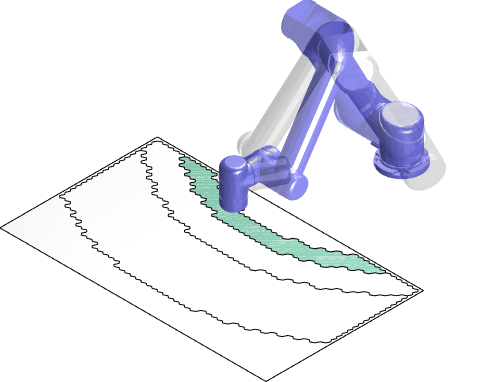
\includegraphics[width = 0.15\textwidth]{square_example/simple_example_merged_545}
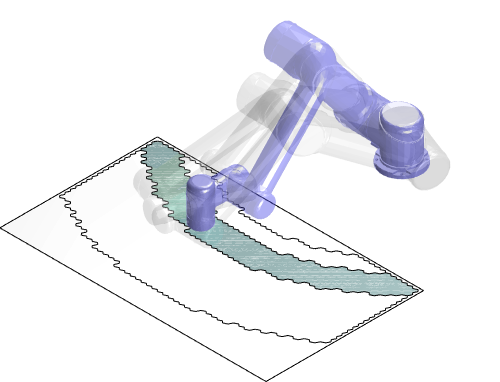
\includegraphics[width = 0.15\textwidth]{square_example/simple_example_merged_551}
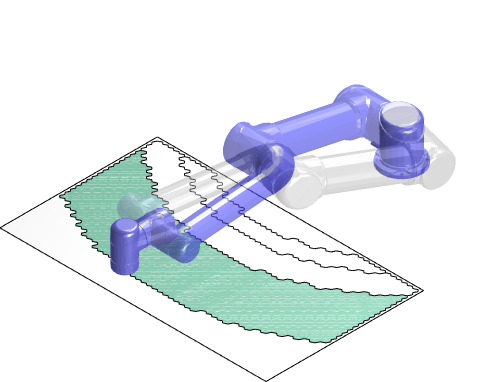
\includegraphics[width = 0.15\textwidth]{square_example/simple_example_merged_565}
\caption{Illustration of different IK solutions for covering a same points. The vivid configurations show one kinds of configurations with shoulder-right, wrist-unflipped. There are also two kinds of configurations (with shoulder left/right and wrist flipped) that are usable. However, they can only cover the middle part of the reachable area. }\label{figsquare}
\end{figure}

\begin{figure}[t]
\centering
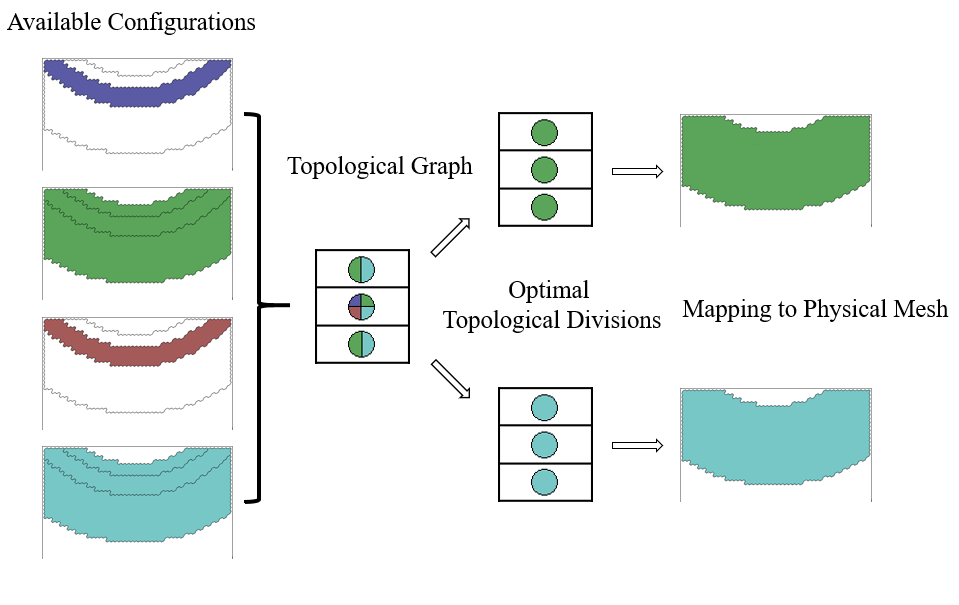
\includegraphics[width = 0.44\textwidth]{flowchart}
\caption{
Flowchart of our algorithm in solving the problem of Figure \ref{figsquare}. 
All configurations are divided into four disjoint sets based on their joint-space continuities, represented by a same color. 
The small circle filled in with color(s) shows all possible colors to paint the corresponding area. The topological graph is created based on the distribution of the colors and being solved. Finally, in this example, we can get two optimal options which both require zero lift-off. 
}\label{flowchart}
\end{figure}


\begin{figure}[t]
\centering
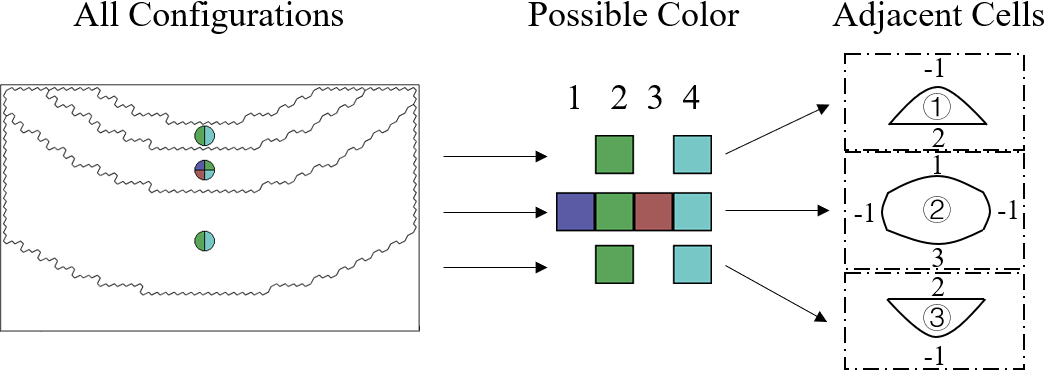
\includegraphics[width = 0.44\textwidth]{square_example/graphcreation}
\caption{
\textcolor{red}{TODO: add correspondence with physical mesh, show the connectivity of the mesh}
The elements of a cell. All colors are indexed. Each cell corresponds to a connected area on the surface of the object and has a list of possible colors. The cell stores the index of its adjacet cell in order. The index of the unreachable area is denoted by $-1$. We use curves to show that the edge is topological but not physical. }\label{figforcolor}
\end{figure}


%\begin{color}{red}
%\subsection{Problem Modeling}\label{sectionmodelling}
%
%Without loss of generality, the input data is a triangular mesh, with all vertices and edges fully known. Then the normal of each vertex and all valid IK solutions to cover it are also known. 
%Since the manipulator is non-redundant, the number of IK solutions for each vertex is finite. 
%Although the mesh is a discretized data structure, we say two vertices are ``continuous'', if there is a list of edges of the mesh connecting them. And we say two configurations are ``continuous'' for the manipulator to reach, if the vertices are continuous, and the distance of these two configurations in the joint-space is near enough. The distance threshold for the continuity is easy to judge, since the manipulability constraint abandones the configurations which are close to the singularities, thus creates an apparent gap between disjoint sets. Typically, just the signs of the joint angles are enough to judge the continuity of two configurations. For example, it is easy to see that three vivid configurations in Figure \ref{figsquare} are continuous, and the greyed out configurations in a same figure are discontinuous pairwise. 
%
%First, we assign the color of all configurations. Starting from an unassigned configuration, using a floodfill-like algorithm on the mesh, all configurations which are continuous with the chosed one are easy to find and are assigned with a same number, which is the index of the corresponding color. After repeating the assignment process, all configurations have a color, and the continuous configurations have a same color. 
%Note that the IK solutions for the same vertex must have different colors. 
%So it is suitable to show the distribution of a color through drawing them on the mesh. For example, Figure \ref{flowchart} shows the distribution of four colors of the example in Figure \ref{figsquare}.
%
%Second, we divide the mesh into several ``cells'', with each vertex belonging to a cell. The cell is a connected open region containing all vertices which are continuous and can be covered through same kinds of colors. 
%For the generation of a cell, we pick up an unassigned vertex, using a floodfill-like algorithm to find all continuous vertices which have same kinds of colors. 
%These vertices belongs to a single cell. In Figure \ref{flowchart}, we draw a small circle filled in with multiple colors to show the possible colors for a cell. After repeating the process, all vertices are assigned. 
%
%Third, after the creation of all cells, we say there is a topological edge between two cells, if there is a physical edge of the mesh which connects two vertices from different cells. 
%We may see the intersection of topological edges in the following figures, but note that they are formally drawed, since each edge connects only two vertices which are impossible to belong to three or more different cells. 
%In all, the structure of the topological graph is uniquely decided by the mesh. 
%
%Finally, the cell records the possible colors for covering the points and the index of its adjacet cells in order, see Figure \ref{figforcolor}. 
%Note that in practical application, since the area of the surface is finite, and each cell must have least size to keep the decomposition meaningful, the number of cells must be finite. 
%
%After creating the topological graph, the original problem is equivalent to painting all points with one of their available colors, ensuring the minimum pieces of colors. And for a fully-filled graph, the color of a point uniquely specifies one of the valid IK solutions to cover it. 
%\end{color}

%\begin{color}{blue}
%\section{Problem Modeling with Symbols}
%\subsection{Problme Statement}
%Same as above.
%\subsection{Independence from the physical coverage path}
%Same as above.
\subsection{Problem Modeling}
First, we define some symbols. Let $\mathscr{C}$ be the set of all valid configurations and $M$ be the set of all reachable points on the surface. The pose of the EE is also denoted by $M$ since there is an one-to-one correspondence between the pose of the EE and the point on the surface, so we do not distinguish them. 

Second, the \textit{color} in Figure \ref{fig1} has significant meaning which deserves formal definition. In mathematical language, the joint-space continuity of two configurations is an equivalence relation (a reflexive, symmetric and transitive relation). Denote the equivalence relation by $\sim$, then each element in the quotient set $\mathscr{C}/\sim$ corresponds to an unique color. 
Now we show the assignment of the color in usual language. 
Given a configuration $p \in \mathscr{C}$ covering $m\in M$, following the joint-space continuity, there exist a neighborhood $(p\in)U_p\subset \mathscr{C}$ that can be reached continuously (without lift-off) from $p$, covering a piece of surface $(m\in )V_{m}\subset M$. 
See Figure \ref{figsquare}, the poses of the manipulator in vivid color can be reached continuously. If any of them is chosen as $p$, then all of them are in $U_p$. 
Assume there are some other unassigned configurations, i.e., $\mathscr{C}\backslash U_p\neq \varnothing$, we choose another one $p'\in \mathscr{C}\backslash U_p$, then it specifies another set $V_{m'}\subset M$. Of course $V_{m'} \cap V_{m} = \varnothing$.
After continuing this process, all configurations are assigned. Then $\mathscr{C}$ is divided into (finite, where we omit the strict proof) number of disjoint sets, denoted by finite number of different colors. 

Third, the \textit{cell}, which is defined on the task-space, the same as that of the conventional cellular decomposition methods, but has a property of homogeneity. 
The basic observation is that the IK mapping shown in Figure \ref{fig1} is injective in each branch. 
The multiple IK solutions appear when the inverse trigonometric function returns multiple solutions. Corresponding to the physical meaning of the 5DOF manipulator, the multiple solutions of the elbow joint causes ``elbow-up/elbow-down'', etc.  
Without strict proof, there exist a joint-angle leading to a singularity in between (``elbow-straight'' in this case). 
%So there does not exist a joint-space path connecting two IK solutions of a same pose of EE without visiting a singularity. 
For example, in each subfigure of Figure \ref{figsquare}, the greyed out configurations have the same pose of the EE with the vivid one, so they must be assigned with different colors. 
\begin{color}{blue}
The injectivity of each branch of the IK motivates us to map the property of joint-space continuity back to the surface, and thus the process of the algorithm can be visualized through drawing color on the surface. % <ty> I used here. 
\end{color}
For example, in Figure \ref{flowchart} we know that $\mathscr{C}$ is divided into 4 disjoint sets. 
Since different IK solutions possess distinct colors, the available colors for points can be used to classify them. Let $\{c_i\}, i = 1, n$ be all colors, then for two points $m_1, m_2\in M$ with their sets of available colors $c_{m_1} = \{c_{11}, \cdots, c_{1i}\}, c_{m_2} = \{c_{21}, \cdots, c_{2j}\}$, we say that $m_1$ and $m_2$ belong to a same cell if and only if 
$$\left\{
\begin{aligned}
& m_1 \mbox{ and } m_2 \mbox{ are connected}\\
& \{c_{11}, \cdots, c_{1i}\} = \{c_{21}, \cdots, c_{2j}\}
\end{aligned}
\right.$$
Typically, for the triangular mesh in our case, the connectivity is provided by the edges of the mesh. Figure \ref{flowchart} shows the creation of the cells. 

Finally, a topological graph is created, whose element is all cells. Each cell possesses an index, records the possible colors and the indices of its adjacet cells in order, like Figure \ref{figforcolor}. 
Note that since the area of the surface is finite, and each cell must have least size to keep the decomposition meaningful, the number of cells must be finite. 
After creating the topological graph, the cellular decomposition process is transformed to painting all points in a graph with one of their available colors.
The number of pieces in the graph means the number of coverage path segments, where discontinuities are required in between. So the optimal cellular decomposition problem is transformed to the painting problem ensuring the minimum pieces of colors. 
For a fully-filled graph, the distribution of the colors specifies a cellular decomposition ensuring no lift-off required in each cell, and the choice from all IK solutions at all points are uniquely specified by the corresponding color. So finally the problem is transformed to finding a color scheme for the graph ensuring least number of pieces.
%\end{color}

\section{Enumerative Solver}\label{sectionenumerativesolver}
The difficulty of solving the coloring problem is that, although the points are gathered into a same cell, they can be filled in with different colors, 
instead of only being seen as a whole and drawn with a single color, see an easy counter-example in Figure \ref{figsimpleexample}. 
We observe that the structure of the graph reflects in the connectivity of the topological edges, which is proved having only finite possible situations in \ref{subsectionproof}. 


\begin{figure}[t]
\centering
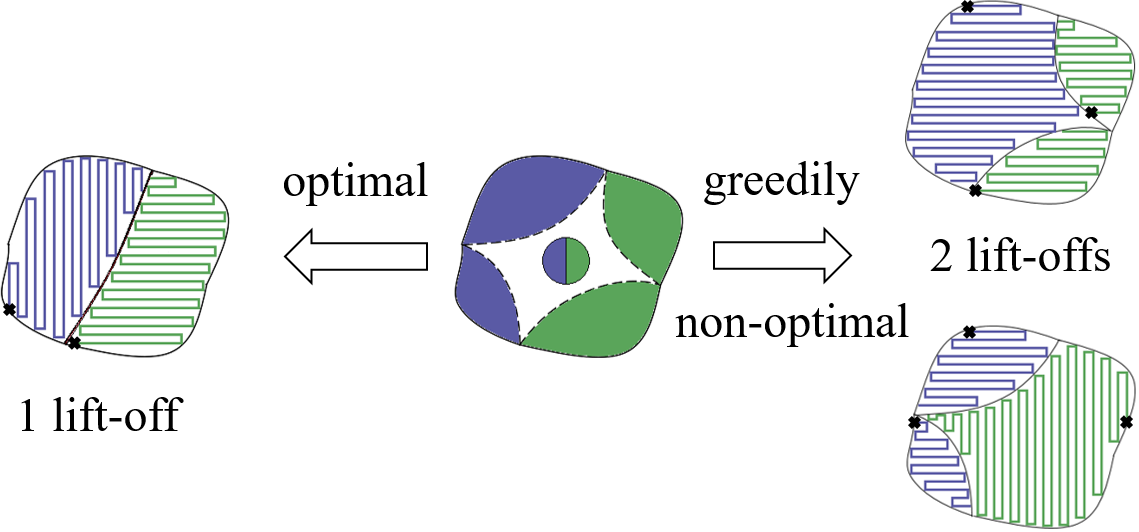
\includegraphics[width = 0.4\textwidth]{simple_example/simple_3}
\caption{
In this graph, only the middle cell still needs solving. 
Whatever pure color filling into the middle cell, it requires an extra lift-off. Instead, if it is cutted into two parts, with two sub-cells filled in with different colors, only $1$ lift-off is required which reach optimality. 
}\label{figsimpleexample}
\end{figure}


In this section, we prove the finiteness of the number of divisions and introduce the enumerative solver through the example of solving a single cell with all its adjacent cells having been colored. We show that the simple cells with less than $4$ topological edges can be enumeratively solved, and there are finite number of manners to divide a complicated cell into several simple cells, hence any cell can be solved. 

\subsection{Finiteness of Divisions}\label{subsectionproof}
Since any path starting and ending at the boundary of a cell will divide the cell into two parts, there are infinite many physical solutions of dividing a cell into parts. However, there are only finite classes of them in the view of topological structure, because of the equivalence of physical divisions in the number of lift-offs. 

See Figure \ref{figproof}(a), we show that the cutting paths which start or end at an ordinary point on some edges are unnecessary. 
Let a cutting path ends at an ordinary point of the edge connecting cell 3. From the definition of a cutting path, it implicitly enforces cell 1 and cell 2 having different colors. Then we may assume $1=3$ or $2=3$ (when $1\neq 3$ and $2\neq 3$ the division is trivial), which, however, is equivalent to two other cutting paths that start at the endpoint of the edge. Do the same discussion on the other endpoint of this cutting path, we know that it is complete to only consider all cutting paths which start and end at the endpoint of some edges.  


See Figure \ref{figproof}(b), we show that the cutting paths which go across some edges are unnecessary. Let a cutting path go across the edge that connects cell 4. 
Then it can be continuously transformed onto the edge without changing the cost. 
This division enforces the constraint of color that $3\neq 4, 3\neq 5, 3\neq 6$. However, it prevents cell 5 and cell 6 from being colored together, because they are separated physically by the cell 3, which may increase the cost and is not optimal. So we can directly discard the cutting paths which go across edges. 

See Figure \ref{figproof}(c), we show that the cutting paths need not go across each other. When two cutting paths intersect, we can change the belonging of the path segment, and then the cutting paths can be continuously transformed onto the existed topological edges. So it is complete to discard the choices of cutting paths which have intersections. 


\begin{figure}[t]
\centering
\subfigure[The unnecessity of having a cutting path which starts or ends at an ordinary point of a topological edge. ]{
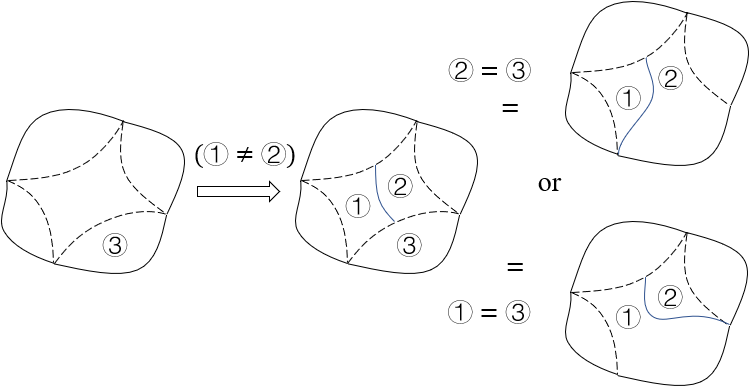
\includegraphics[width=0.4\textwidth]{proof/equiv_cutting_path}
}
\subfigure[The unnecessity of having a cutting path going across an edge. ]{
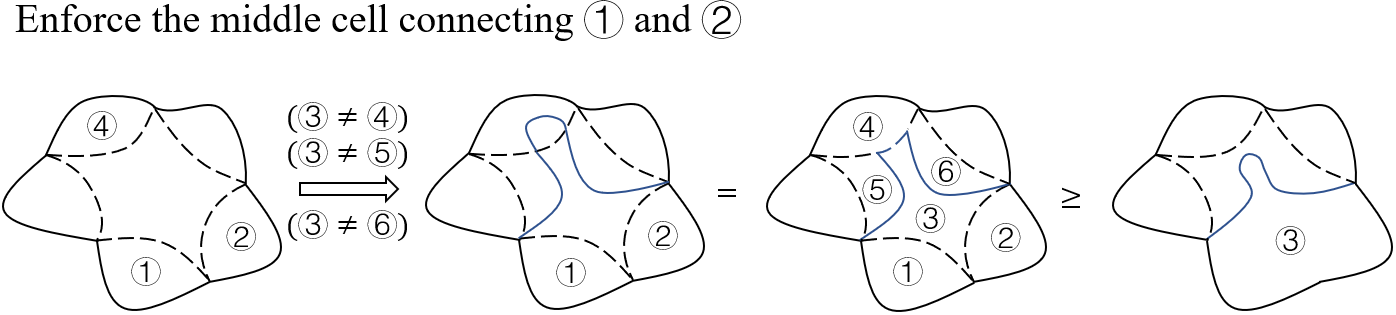
\includegraphics[width=0.48\textwidth]{proof/equiv_cutting_path2}
}
\subfigure[The unnecessity of intersecting two cutting paths.]{
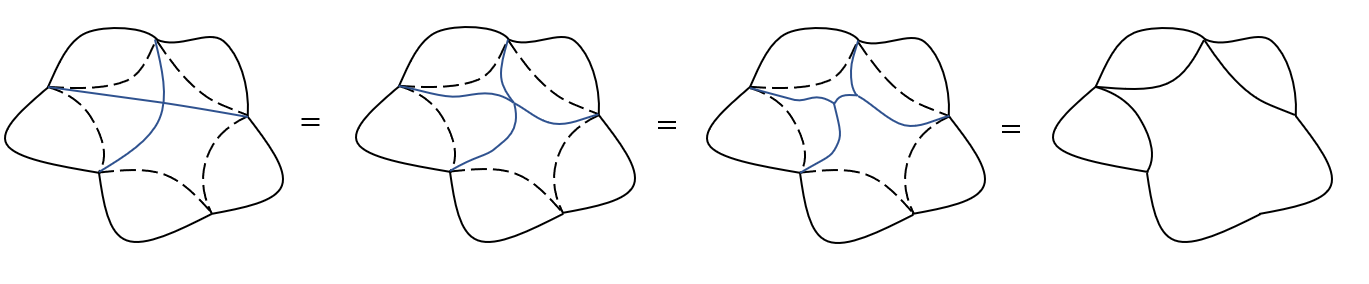
\includegraphics[width = 0.48\textwidth]{proof/equiv_cutting_path3}
}
\caption{Some physical divisions that are unnecessary or non-optimal. }\label{figproof}
\end{figure}

In conclusion, we only need to consider all cutting paths which start and end at the endpoint of some topological edges and do not go across each other. Hence, the total number of topological divisions is finite and we just need to go through all possible divisions. 


\subsection{Solution of Simple Cells}
The following kinds of cells are so simple that can be solved directly without further divisions:

(1) The cells containing less than four edges,

(2) The cells with only one possible color,

\noindent
because the cells of (1) cannot be divided further into several cells with less number of topological edges, and the cells of (2) have no other choice of color. We enumerate all possible topological divisions of a 3-edge cell (which is the most complicated case for direct enumeration) in Figure \ref{figeasycell3}. We use a binary number to represent the connectivity of the edges, $1$ for connection, $0$ for disconnection. It is easy to see that there are at most $8$ situations.

\begin{figure}[t]
\centering
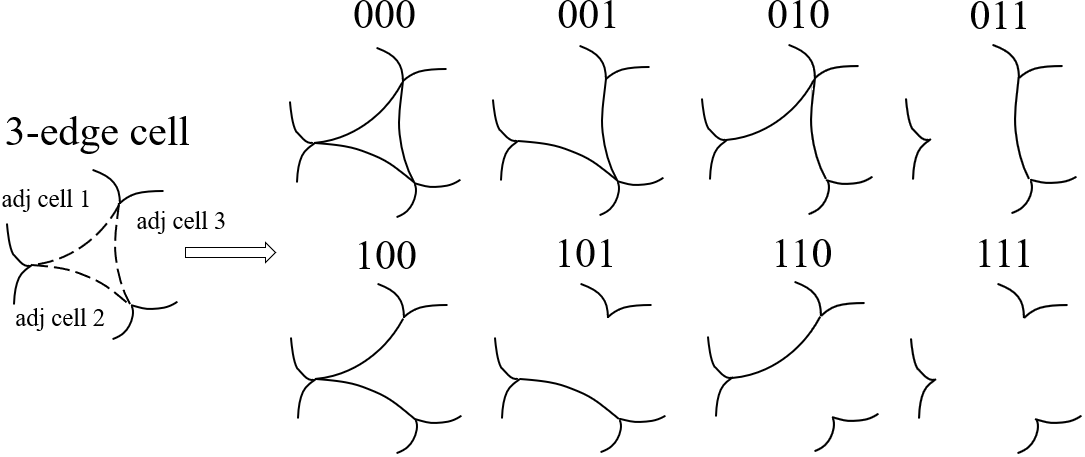
\includegraphics[width = 0.44\textwidth]{easycell/cell3}
\caption{All possible divisions of a 3-edge cell, which is the most complicated situation that need not further divisions. Although some of them are the same in the topological structure (e.g., $001, 010$ and $100$), or the division is impossible (e.g., we enforce $011$ but the cell 1 and cell 2 do not have a same color), it has already been a finite problem, so we omit the description of further simplification. }\label{figeasycell3}
\end{figure}


\subsection{Solution of Complicated Cells}

Following the idea of solving a simple cell, we use a binary number of length $n$ to represent the connectivity of an $n$-edge cell, $1$ for connection, $0$ for disconnection and $\times$ for the unspecified state. 
The continuous $1$s imply that part of this cell must be painted with the same color as that of the adjacent cells which the $1$s specify. 
The $0$ means that the topological edge between the cell and the corresponding adjacent cell is keeped so that the colors must be different. 
The unspecified states $\times$ imply the generation of a sub-cell. An example of solving a 4-edge cell is shown in Figure \ref{figeasycell4}. Through specifying the position of $1$s, there are less than $2^n\times m$ branches for an $n$-edge cell with $m$ possible colors, so the problem is finite. The distinguishment between $0$ and $\times$ will be given in subsection \ref{subsectiondiscussion}.

\begin{figure}[t]
\centering
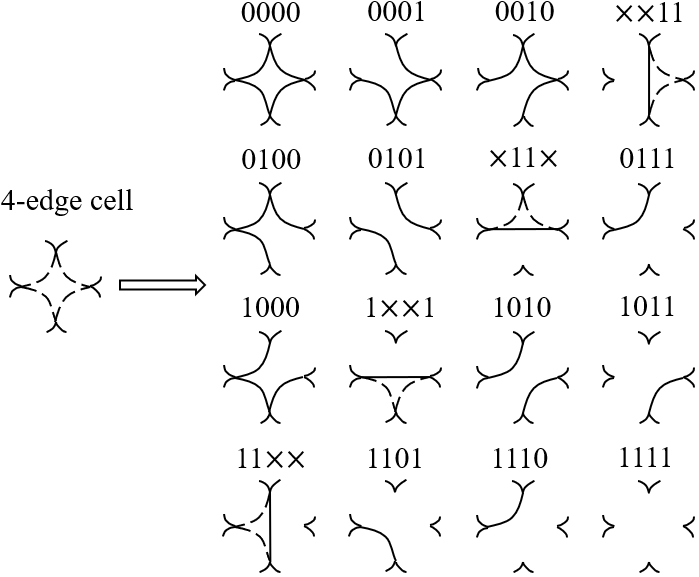
\includegraphics[width = 0.4\textwidth]{easycell/cell4}
\caption{The $2^4$ possible divisions of an 4-edge cell. For the cell which has more than 3 edges, the sub-cell may be created. In this figure, the connectivities that correspond to generating a sub-cell is $\times\times11, \times11\times, 1\times\times1, 11\times\times$. }\label{figeasycell4}
\end{figure}

\subsection{Discussion of Creating Sub-Cells}\label{subsectiondiscussion}
When there exist such number lists in the connectivities: 
$$1\times\times1, 1\times\times\times1, \cdots$$
the cell is divided into parts whose colors are enforced to be different, so called sub-cells.
See the case of $\times\times11, \times11\times, 1\times\times1, 11\times\times$ in Figure \ref{figeasycell4}. The original cell becomes a new one with fewer edges, becasue some edges are replaced by a single edge. We use the bracket $(\cdots)$ in the binary number of the original cell to represent the generation of sub-cells.
Do the same division for the sub-cells, any $n$-edge cell can be continuously divided into a set of 3-edge cells and then be solved enumeratively. 

Since the sub-cell is generated from an original one, there are extra constraints on its connectivity specified by the previous division. However, these constraints cannot change this problem into one with polynomial time solution, so we just give some examples among them:

(1) Single $\times$ cannot form a sub-cell, because 
$$\cdots 1\times 1\cdots = \cdots 101\cdots \mbox{ or }\cdots 111\cdots$$
but both conditions of the right side are considered in other branches. This is why there is no $\times$ in Figure \ref{figeasycell3}.  

(2) The $0$s can be freely moved outside the bracket, because of the equivalence 
$$\cdots\times1(0\times\cdots\times1)1\times\cdots = \cdots\times10(\times\cdots\times1)1\times\cdots$$
and the same is true for the right bracket based on the symmetry of the number list, because the cutting graph makes sense only when the inner boundary two numbers are $1$s. See Figure \ref{figconstraint}. This is why no brackets in Figure \ref{figeasycell4}.

(3) The new topological edge created by the cutting path must be keeped (always $0$, impossible to be $1$ or $\times$) because it is manually created. Hence, for the entire problem, no extra possiblities appear after the divisions 

\begin{figure}[t]
\centering
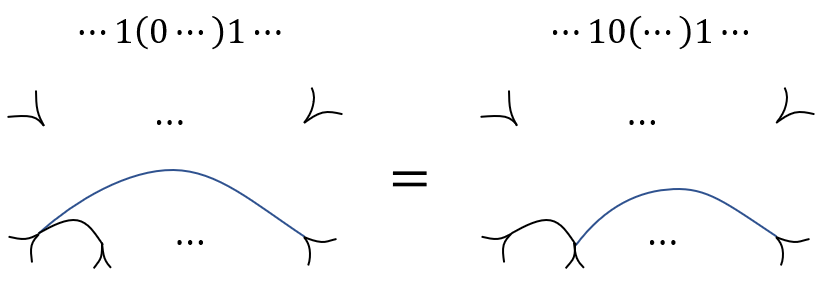
\includegraphics[width = 0.3\textwidth]{proof/equiv_zero}
\caption{The equivalence of moving the $0$ outside the bracket. In order to reduce the number of edges of the sub-cell, we always enforce the sub-cell looking like the right side. }\label{figconstraint}
\end{figure} 



\section{Iterative Solver}\label{sectioniterativesolver}

%\begin{color}{blue}
%The solving process is iteratively executed. In each iteration, the algorithm chooses an unsolved cell, finds its all possible solutions and creates a branch for each possible solution. In each branch, the chosed cell is filled in with the specified color (so it will not change any more). 
%Then, in the next iteration, the algorithm chooses an unsolved branch, chooses an unsolved cell in it and does the same steps as before. 
%Finally, after iteratively solving, each branch becomes a valid scheme for coloring or returns with a contradiction. 
%The algorithm runs like the deepest-first-searching (DFS) algorithm so that the memory requirement is not high. 
%\end{color}

\subsection{Iteration Process}
Regarding the enumerative solver as a basic step, we iteratively solve the graph. 
Starting from a fully-unpainted graph, we choose an unsolved cell and enumerativelly solve it. 
Assume that the cell has $n$-edges with $m$ possible colors, there are at most $2^n\times m$ possible divisions. We create a branch for each possible solution of the chosed cell, and in each branch the chosed cell is filled in with the specfied color (so it will not change any more). 
In the next iteration, we choose an unsolved branch, choose an unsolved cell in it and do the same steps as before. 
Note that the constraints given by the solved adjacent cells hugely restrict the possible solutions, because the state of an edge resticts the connectivity of the cells on both side. 
After iterative execution, all branches reach a contradiction or a valid coloring scheme. A valid coloring scheme for the graph uniquely specify the configuration to polish each point among its valid IK solutions. 
The algorithm runs like the deepest-first-searching (DFS) algorithm so that the memory requirement is not high. 
Since the execution is an exhaustive searching, all optimal physical cellular decompositions must be homeomorphic to one of our result schemes, with the position of the physical boundaries of the cells slightly different to the physical ones.

\subsection{Calculation of Cost}
The physical meaning of the cost for a (partly filled) graph is the number of pieces of color in the current graph. 
Describing the formula incrementally, after we solve a cell, 

(1) If its connectivity is all zero, then the cost will increase $1$ after coloring this cell, because this cell forms a new piece.

(2) If its connectivity has only one $1$ connecting a solved cell, then the cost will not change, because this cell can be filled together with the connected adjacent cell. 

(3) For its connectivity with $i$ $1$s, note that there may exist multiple edges which connect the same adjacent cell (See Figure \ref{figcost}). In order to be consistent with the physical meaning of the cost, if these edges connect $j$ distinct solved cells, then the variation of cost is 
$$\Delta cost = 1-j$$


\begin{figure}[t]
\centering
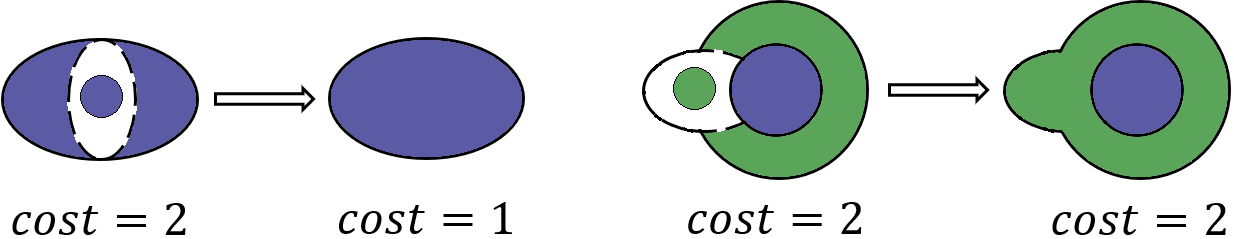
\includegraphics[width = 0.4\textwidth]{proof/costcal}
\caption{Left: the middle cell connects two distinct cells, so the cost variation is $1-2 = -1$. Right: two edges connect with the same adjacent cell, then the cost variation is $1-1 = 0$ but not $1-2 = -1$.}\label{figcost}
\end{figure}

\section{Experimental Results}\label{sectionexperiment}

Our algorithm works on any non-repetitive coverage task using non-redundant manipulators in any dimension. 
In this paper, experiments are taken by using a 5DOF manipulator to polish the surface of an object. And the manipulator should cover all reachable points even if it cannot fully cover the surface. 

First, we discuss the proposed algorithm using behind other cellular decompositions, from which the proposed algorithm can be seen as a tool for the evaluation of other cellular decomposition algorithms. 
Then, in the first simulated experiment, a hemispherical object is polished at different poses, one casually placed and the other being designed precisely. Through calculating the least required number of lift-offs, the quality of the placement of the object can be evaluated. 
In the second simulated experiment, we show that the proposed algorithm directly contributes to the choice of the configurations. We show some non-optimal configurations, which will never be chosed through applying the proposed algorithm.
Finally, in the real-world experiment, the manipulator polishes a wok following a manually generated physical coverage path under the presence of the obstacles, which proves the applicablity of the proposed algorithm. 
\begin{color}{blue}
The video of the real-world experiment is here: 
\end{color}

Unless otherwise stated, the environment contains only the manipulator, the object and the ground plane. 
And note that all figures in this section are just an example of the optimal solutions. 
As we have discussed before, there are infinite many physical cutting paths of decomposition that result in same number of lift-offs of the EE, and the choices of the physical coverage paths within each cell are also arbitrary.


\subsection{Calculating least number of discontinuities for other methods}
Since all cellular decompositions divide the whole reachable region into parts, implicitly imply discontinuities between cells. Then, the original problem can be solved through finding coverage path in each cell, and the result path is the concatenation of the path segments in each cell using paths where the EE is lifted off. Let a cellular decomposition methods divides the surface into $n$ parts, then $n-1$ lift-offs are required. However, notice that tracking the coverage path in each cell still requires lift-off, denoted by $p_i$. Then the least number of lift-offs a given cellular decomposition is 
$$n-1 + \sum\limits_{i = 1}^n p_i$$ 
where $p_i$ can be calculated through using the proposed algorithm in the $i-$th cell. 

To show the optimality of the proposed algorithm, we apply it to the cellular decomposition created by itself. Since each cell is guaranteed polishable with no lift-off, $p_i = 0, \forall i$. Moreover, the number $n$ is optimal since we use haustive seraching strategy. Hence, the proposed algorithm certainly outperforms other methods in the sense of the number of lift-offs. 



\subsection{Covering a hemisphere}
In this experiment, through the polishing task of a hemisphere shape object, we show that the number of lift-offs provided by our algorithm can evaluate the quality of the placement of the object (or the manipulator). 

See Figure \ref{figflatwise}, a common scene is that the object is casually placed (e.g., on an automated production line) and a coverage path is designed, since there is no apparent criterion on the quality of the placement. However, the proposed algorithm shows that such a placement of the object requires at least $3$ lift-offs, but still fails in full coverage (the farthest area is unreachable), which is equivalent to at least $4$ lift-offs. 
Instead of the usual setting, see Figure \ref{figsloped}, if we precisely design the pose of the object (obliquely at $(0.7m, 0.1m, 0.08m)$), then not only the least number of lift-offs decreases to $2$, but the manipulator can fully cover the surface, which performs much better than the scene in Figure \ref{figflatwise}. Hence, the required number of lift-offs guides the user to try different poses of the object (or the manipulator) to have better performance on coverage. 


\begin{figure}[t]
\centering
\subfigure[]{
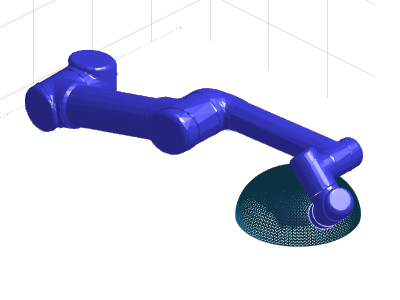
\includegraphics[width = 0.10\textwidth]{exp_semi_ellipsoid/casual_demo}
}
\subfigure[]{
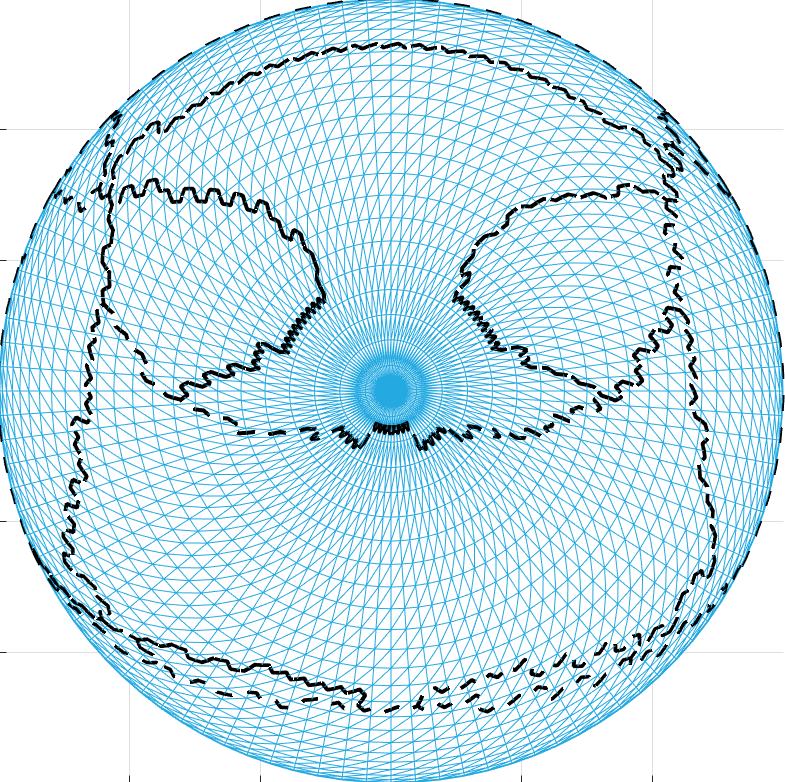
\includegraphics[width = 0.10\textwidth]{exp_semi_ellipsoid/casual_init_graph}
}
\subfigure[]{
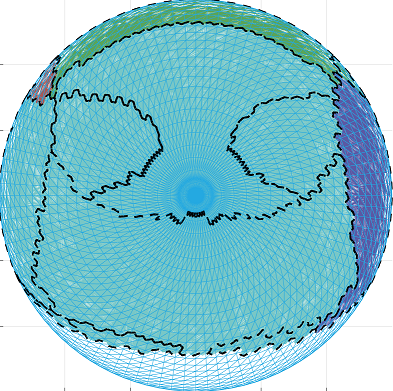
\includegraphics[width = 0.10\textwidth]{exp_semi_ellipsoid/casual_result_graph}
}
\subfigure[]{
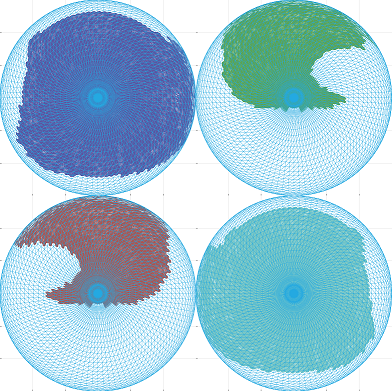
\includegraphics[width = 0.10\textwidth]{exp_semi_ellipsoid/casual_comb}
}
\caption{(a) The object is casually placed. (b) The initial graph. (c) One optimal solution which requires 3 lift-offs, but the manipulator still cannot fully cover the farthest part of the mesh (the top area in the figure). (d) The reachable area of four kinds of valid configuration chosed by the optimal solution in (c). 
}\label{figflatwise}
\end{figure}
\begin{figure}[t]
\centering
\subfigure[]{
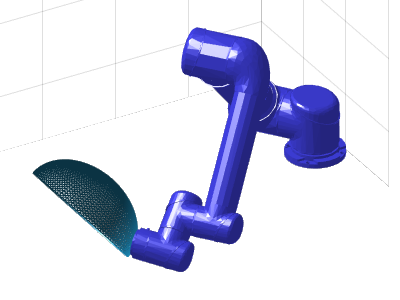
\includegraphics[width = 0.1\textwidth]{exp_semi_ellipsoid/design_demo}
}
\subfigure[]{
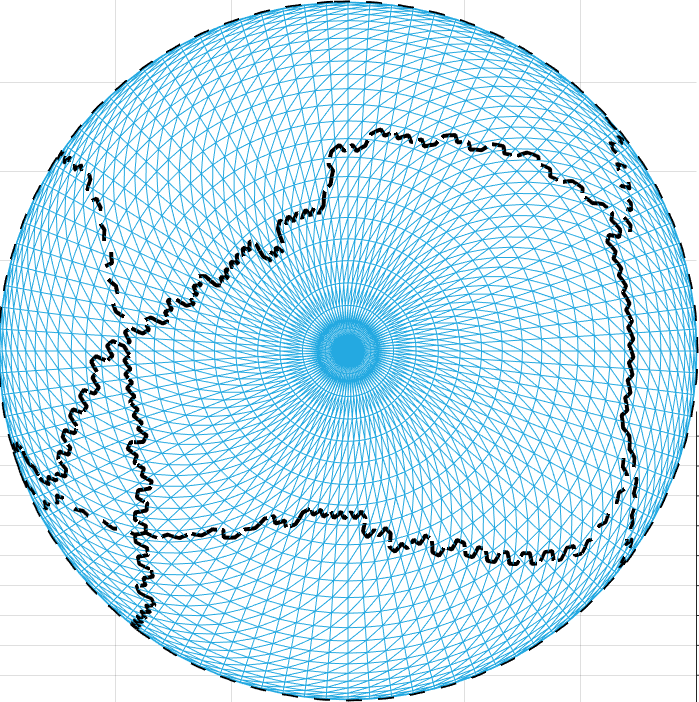
\includegraphics[width = 0.1\textwidth]{exp_semi_ellipsoid/design_init_graph}
}
\subfigure[]{
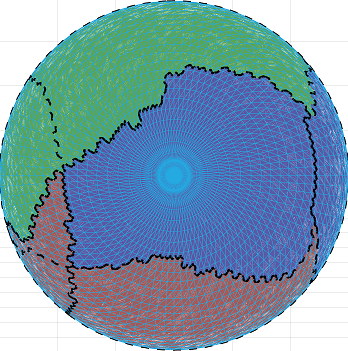
\includegraphics[width = 0.1\textwidth]{exp_semi_ellipsoid/design_result_graph}
}
\subfigure[]{
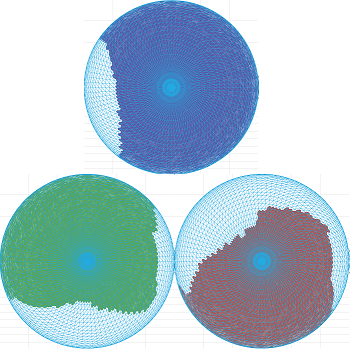
\includegraphics[width = 0.1\textwidth]{exp_semi_ellipsoid/design_comb}
}
\caption{(a) The object is placed obliquely. (b) The initial graph. (c) One optimal solution which only requires 2 lift-offs but realizes full coverage. (d) The reachable area of three kinds of valid configurations which are chosed by the optimal solution in (c). 
}\label{figsloped}
\end{figure}


\subsection{Covering a pipe}
In this subsection, through the polishing task of a half pipe, we show that the proposed algorithm can clearify the unnecessary configurations, avoid the ``trapped'' configurations which cause extra lift-offs. 

The pipe is placed obliquely. Althrough the object is common, the normal of its surface varies for $\pi$ rad, which causes difficulty for the manipulator. We show the initial graph and directly give its optimal solution in Figure \ref{fighalfpipe}. The optimal solution of this coverage task requires only $1$ lift-off. 

There are many valid configurations which directly leads to non-optimality, because they just cover some points which have many IK solutions but break the connectivity of the uncovered region. 
See Figure \ref{figthreeexamplepose} for an example of the distinguishability of the trap configurations. 
The first kind of configurations and the third one are finally chosed by one of the optimal solutions shown in Figure \ref{fighalfpipe}. 
The second kind of configurations can cover large area without lift-offs, which is very likely to be chosed if the IK solutions are chosed randomly or greedily. However, it cannot cover the corners of the mesh (which are eventually covered by the other two ones). Once any configurations belonging to the second kind is chosed, after the coverage of the middle part of the pipe, sooner or later it has to waste two lift-offs to finish the full coverage, which leads to non-optimality. The proposed algorithm provides all optimal solutions where none of them uses the second color, thus prevent from choosing these non-optimal configurations. 
\begin{figure}[t]
\centering
\subfigure[]{
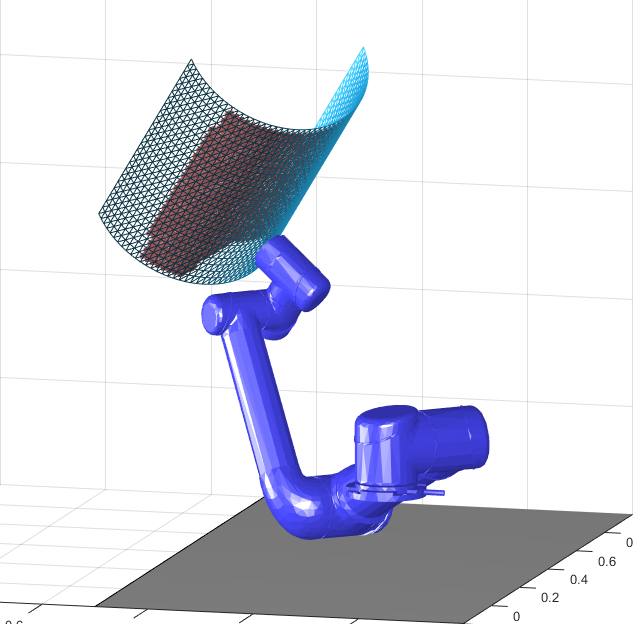
\includegraphics[width = 0.14\textwidth]{exp_pipe/demo}
}
\subfigure[]{
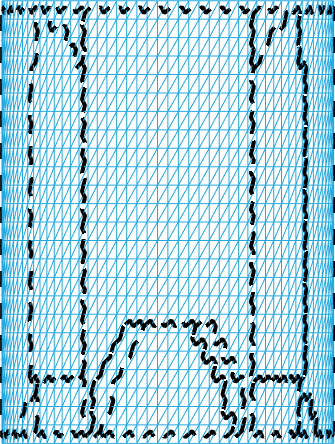
\includegraphics[width = 0.14\textwidth]{exp_pipe/init_graph}
}
\subfigure[]{
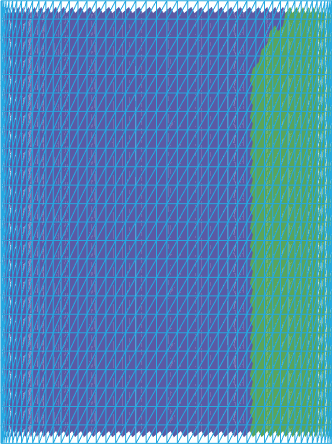
\includegraphics[width = 0.14\textwidth]{exp_pipe/result_graph}
}
\caption{(a) The manipulator is polishing the top-right corner where can only be polished through kinds of configurations. (b) The initial topological graph of this problem. (c) One optimal solution which requires 1 lift-off.}\label{fighalfpipe}
\end{figure}

\begin{figure}[htb]
\centering
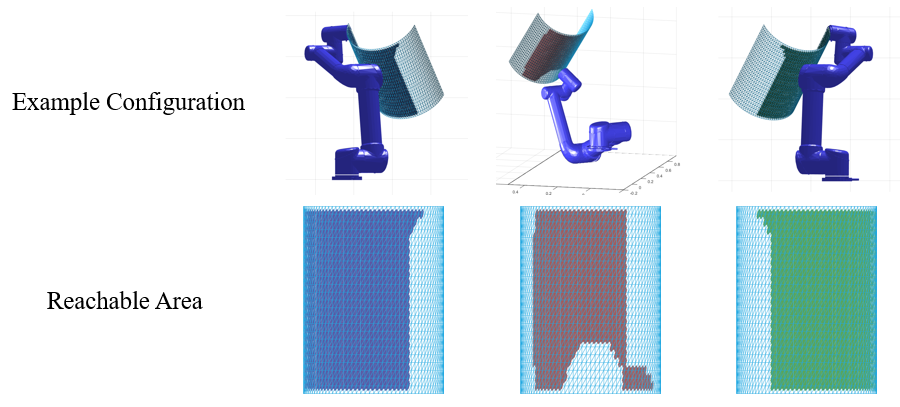
\includegraphics[width = 0.4\textwidth]{exp_pipe/three_example_pose}
\caption{Example of three different kinds of configurations and the distribution of their reachable area. Once any configuration belonging to the second kind is mistakenly chosed to cover any area of the surface, sooner or later we have to change to the first one and the third one to finish the full coverage of the surface, which wastes an unnecessary lift-off.}\label{figthreeexamplepose}
\end{figure}

\subsection{Real World Experiments with Presence of Obstacles}

In this subsection, we use a manipulator polishing the outer surface of a wok to show a physical coverage path generated based on the proposed cellular decomposition method. 
The physical coverage path uses simple back and force motions, whose generation is not part of our concern. The concatenation between paths in different cells are created by demonstration. 
The manipulator is UR5, with its last joint abandoned, equivalent to 5DOF, which is non-redundant. 
Since the hybrid position/force control is beyond our contribution, we do not envolve the real contact. 

See Figure \ref{fig_realworld_no}, the nearest and farthest part of the wok are unreachable. 
Considering the two points shown in Figure \ref{fig_realworld_no}(d)(e), the manipulator has to keep its wrist ``above'' its fore-arm in order to avoid collision between them, which leads to the requirement of both shoulder-left configurations and shoulder-right configurations. 
The total number of lift-off is $1$. Since each color covers some points which only have one possible color, the solution is definitely optimal. Note that any division keeping the connectivity is optimal, so we may just divide the surface through the middle. 

See Figure \ref{fig_realworld_with}, the manipulator is obstructed by a cylindrical obstacle. Since the obstacle may collide with the upper-arm, fore-arm or the EE, and the wrist may collide with the fore-arm, to avoid all collisions, the least number of lift-offs is 2. Similarly, each color covers some points which only have one possible color, so the solution is also optimal. 

\begin{figure}[t]
\centering
\subfigure[]{
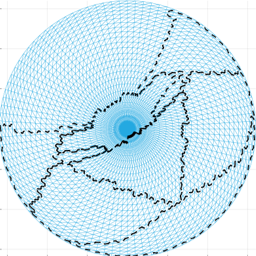
\includegraphics[width = 0.14\textwidth]{real_world_exp/no_obstacle_initial_graph}
}
\subfigure[]{
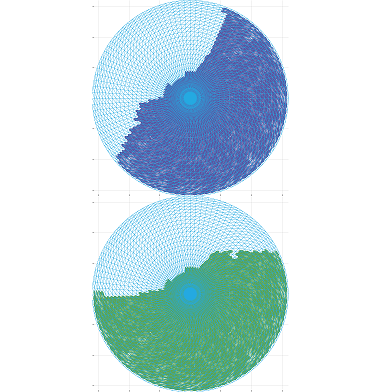
\includegraphics[width = 0.14\textwidth]{real_world_exp/no_obstacle_comb}
}
\subfigure[]{
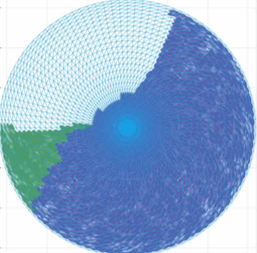
\includegraphics[width = 0.14\textwidth]{real_world_exp/no_obstacle_result_graph}
}
\subfigure[]{
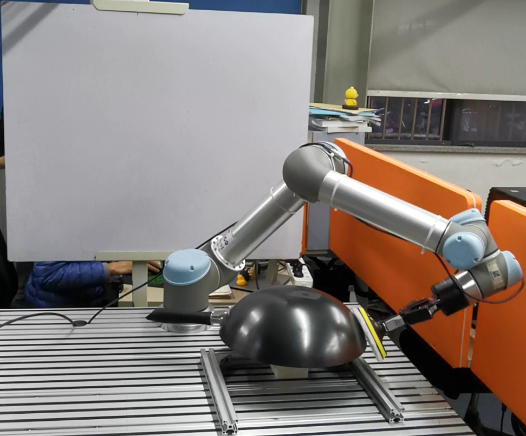
\includegraphics[width = 0.2\textwidth]{real_world_exp/no_obstacle_demo_1}
}
\subfigure[]{
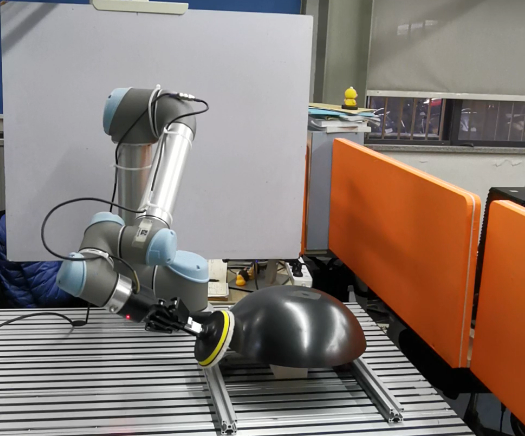
\includegraphics[width = 0.2\textwidth]{real_world_exp/no_obstacle_demo_2}
}
\caption{(a) Initial graph. (b) The reachable area of two kinds of configurations which are chosed by the solution in (c). (c) The cutting graph is arbitrary, so we may divide the graph through the middle. (d)(e) Example of the extreme poses of the two kinds of configurations. }\label{fig_realworld_no}
\end{figure}

\begin{figure}[t]
\centering
\subfigure[]{
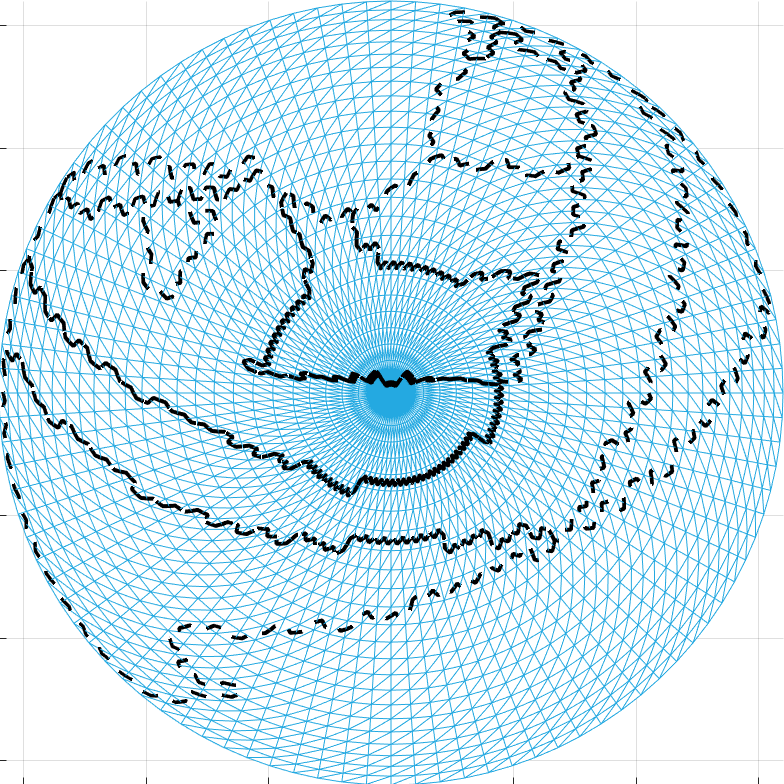
\includegraphics[width = 0.14\textwidth]{real_world_exp/with_obstacle_initial_graph}
}
\subfigure[]{
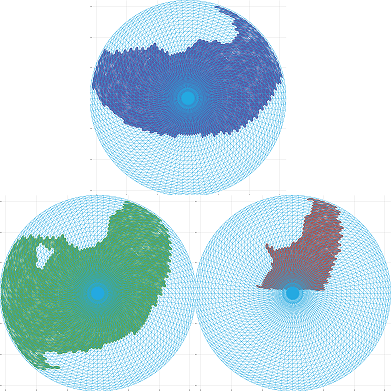
\includegraphics[width = 0.14\textwidth]{real_world_exp/with_obstacle_comb}
}
\subfigure[]{
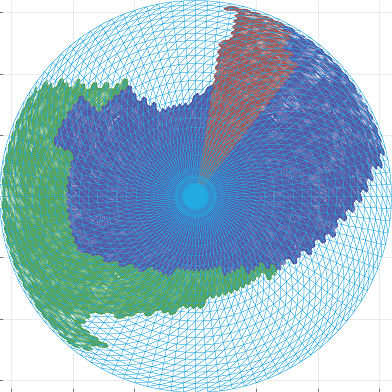
\includegraphics[width = 0.14\textwidth]{real_world_exp/with_obstacle_result_graph}
}
\subfigure[]{
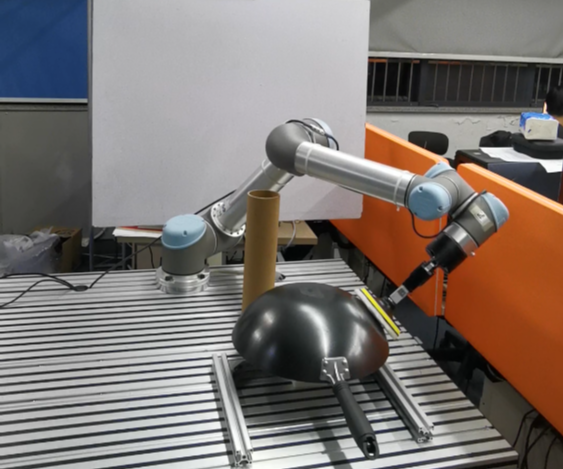
\includegraphics[width = 0.14\textwidth]{real_world_exp/with_obstacle_demo_1}
}
\subfigure[]{
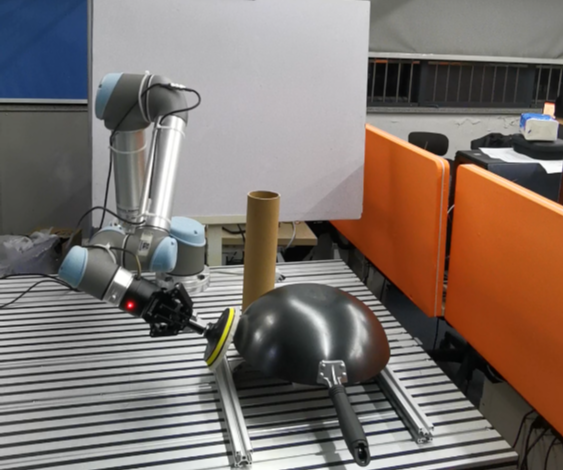
\includegraphics[width = 0.14\textwidth]{real_world_exp/with_obstacle_demo_2}
}
\subfigure[]{
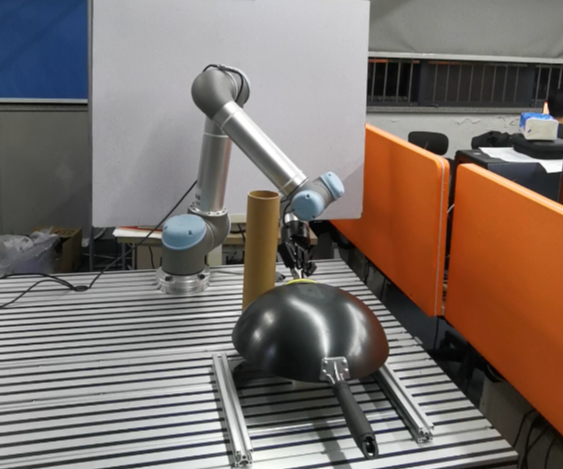
\includegraphics[width = 0.14\textwidth]{real_world_exp/with_obstacle_demo_3}
}
\caption{(a) The initial graph. (b) The reachable area of three kinds of configurations which are chosed by the solution in (c). (c) One optimal solution. (d)(e)(f) Example of the three kinds of configurations, where
(d) The shoulder-left configurations avoid collision between the upper-arm and the obstacle. (e) The wrist is above the fore-arm so that the wrist will not hit the fore-arm. (f) The only valid configuration to cover this point is putting the wrist below the fore-arm. }\label{fig_realworld_with}
\end{figure}

\section{Conclusion}\label{sectionconclusion}
In this paper, we first prove that the least number of the discontinuities is independent to the choice of the coverage path, thus becomes a criterion evaluating the quality of the placement of the manipulator (or the object), which may contribute to the mobile manipulator or the designing of the assembly line. Then, the proposed algorithm provides a novel cellular decomposition strategy, which, after applying the conventional CPP algorithm in each cell, generates the result coverage path containing the least number of discontinuities, which is verified through simulated and real-world experiments. 
Also, as a direct corollary, applied to the result of other cellular decomposition methods, the proposed algorithm can tell the user the least number of discontinuities obeying the given cellular decomposition. 

Because of the transition strategy which is more complicated than usual movement for coverage required by the discontinuities, and due to the unreachabiliy of the optimal coverage path, an NP problem, the optimality criterion of the coverage path that ensuring least number of discontinuities becomes more significant, and reducing the number of discontinuities is practical to reduce the cost of the coverage task, which is solvable through the proposed algorithm. 

In the future, a more complicated situation will be considered, where the initial topological graph contains ring-like cells, which can be broken during the iterative solving process. And the real contact process will be envolved to quantize the energy saving.



% An example of a floating figure using the graphicx package.
% Note that \label must occur AFTER (or within) \caption.
% For figures, \caption should occur after the \includegraphics.
% Note that IEEEtran v1.7 and later has special internal code that
% is designed to preserve the operation of \label within \caption
% even when the captionsoff option is in effect. However, because
% of issues like this, it may be the safest practice to put all your
% \label just after \caption rather than within \caption{}.
%
% Reminder: the "draftcls" or "draftclsnofoot", not "draft", class
% option should be used if it is desired that the figures are to be
% displayed while in draft mode.
%
%\begin{figure}[!t]
%\centering
%\includegraphics[width=2.5in]{myfigure}
% where an .eps filename suffix will be assumed under latex, 
% and a .pdf suffix will be assumed for pdflatex; or what has been declared
% via \DeclareGraphicsExtensions.
%\caption{Simulation results for the network.}
%\label{fig_sim}
%\end{figure}

% Note that the IEEE typically puts floats only at the top, even when this
% results in a large percentage of a column being occupied by floats.


% An example of a double column floating figure using two subfigures.
% (The subfig.sty package must be loaded for this to work.)
% The subfigure \label commands are set within each subfloat command,
% and the \label for the overall figure must come after \caption.
% \hfil is used as a separator to get equal spacing.
% Watch out that the combined width of all the subfigures on a 
% line do not exceed the text width or a line break will occur.
%
%\begin{figure*}[!t]
%\centering
%\subfloat[Case I]{\includegraphics[width=2.5in]{box}%
%\label{fig_first_case}}
%\hfil
%\subfloat[Case II]{\includegraphics[width=2.5in]{box}%
%\label{fig_second_case}}
%\caption{Simulation results for the network.}
%\label{fig_sim}
%\end{figure*}
%
% Note that often IEEE papers with subfigures do not employ subfigure
% captions (using the optional argument to \subfloat[]), but instead will
% reference/describe all of them (a), (b), etc., within the main caption.
% Be aware that for subfig.sty to generate the (a), (b), etc., subfigure
% labels, the optional argument to \subfloat must be present. If a
% subcaption is not desired, just leave its contents blank,
% e.g., \subfloat[].


% An example of a floating table. Note that, for IEEE style tables, the
% \caption command should come BEFORE the table and, given that table
% captions serve much like titles, are usually capitalized except for words
% such as a, an, and, as, at, but, by, for, in, nor, of, on, or, the, to
% and up, which are usually not capitalized unless they are the first or
% last word of the caption. Table text will default to \footnotesize as
% the IEEE normally uses this smaller font for tables.
% The \label must come after \caption as always.
%
%\begin{table}[!t]
%% increase table row spacing, adjust to taste
%\renewcommand{\arraystretch}{1.3}
% if using array.sty, it might be a good idea to tweak the value of
% \extrarowheight as needed to properly center the text within the cells
%\caption{An Example of a Table}
%\label{table_example}
%\centering
%% Some packages, such as MDW tools, offer better commands for making tables
%% than the plain LaTeX2e tabular which is used here.
%\begin{tabular}{|c||c|}
%\hline
%One & Two\\
%\hline
%Three & Four\\
%\hline
%\end{tabular}
%\end{table}


% Note that the IEEE does not put floats in the very first column
% - or typically anywhere on the first page for that matter. Also,
% in-text middle ("here") positioning is typically not used, but it
% is allowed and encouraged for Computer Society conferences (but
% not Computer Society journals). Most IEEE journals/conferences use
% top floats exclusively. 
% Note that, LaTeX2e, unlike IEEE journals/conferences, places
% footnotes above bottom floats. This can be corrected via the
% \fnbelowfloat command of the stfloats package.









% if have a single appendix:
%\appendix[Proof of the Zonklar Equations]
% or
%\appendix  % for no appendix heading
% do not use \section anymore after \appendix, only \section*
% is possibly needed

% use appendices with more than one appendix
% then use \section to start each appendix
% you must declare a \section before using any
% \subsection or using \label (\appendices by itself
% starts a section numbered zero.)
%


%\appendices
%\section{Proof of the First Zonklar Equation}
%Appendix one text goes here.
%
%% you can choose not to have a title for an appendix
%% if you want by leaving the argument blank
%\section{}
%Appendix two text goes here.


% use section* for acknowledgment
\section*{Acknowledgment}


The authors would like to thank...

\bibliographystyle{ieeetr} %% setting the cite style
\bibliography{min_removal}

% Can use something like this to put references on a page
% by themselves when using endfloat and the captionsoff option.
\ifCLASSOPTIONcaptionsoff
  \newpage
\fi



% trigger a \newpage just before the given reference
% number - used to balance the columns on the last page
% adjust value as needed - may need to be readjusted if
% the document is modified later
%\IEEEtriggeratref{8}
% The "triggered" command can be changed if desired:
%\IEEEtriggercmd{\enlargethispage{-5in}}

% references section

% can use a bibliography generated by BibTeX as a .bbl file
% BibTeX documentation can be easily obtained at:
% http://mirror.ctan.org/biblio/bibtex/contrib/doc/
% The IEEEtran BibTeX style support page is at:
% http://www.michaelshell.org/tex/ieeetran/bibtex/
%\bibliographystyle{IEEEtran}
% argument is your BibTeX string definitions and bibliography database(s)
%\bibliography{IEEEabrv,../bib/paper}
%
% <OR> manually copy in the resultant .bbl file
% set second argument of \begin to the number of references
% (used to reserve space for the reference number labels box)
%\begin{thebibliography}{1}
%
%\bibitem{IEEEhowto:kopka}
%H.~Kopka and P.~W. Daly, \emph{A Guide to \LaTeX}, 3rd~ed.\hskip 1em plus
%  0.5em minus 0.4em\relax Harlow, England: Addison-Wesley, 1999.
%
%\end{thebibliography}

% biography section
% 
% If you have an EPS/PDF photo (graphicx package needed) extra braces are
% needed around the contents of the optional argument to biography to prevent
% the LaTeX parser from getting confused when it sees the complicated
% \includegraphics command within an optional argument. (You could create
% your own custom macro containing the \includegraphics command to make things
% simpler here.)
%\begin{IEEEbiography}[{\includegraphics[width=1in,height=1.25in,clip,keepaspectratio]{mshell}}]{Michael Shell}
% or if you just want to reserve a space for a photo:

\begin{IEEEbiography}{Michael Shell}
Biography text here.
\end{IEEEbiography}

% if you will not have a photo at all:
\begin{IEEEbiographynophoto}{John Doe}
Biography text here.
\end{IEEEbiographynophoto}

% insert where needed to balance the two columns on the last page with
% biographies
%\newpage

\begin{IEEEbiographynophoto}{Jane Doe}
Biography text here.
\end{IEEEbiographynophoto}

% You can push biographies down or up by placing
% a \vfill before or after them. The appropriate
% use of \vfill depends on what kind of text is
% on the last page and whether or not the columns
% are being equalized.

%\vfill

% Can be used to pull up biographies so that the bottom of the last one
% is flush with the other column.
%\enlargethispage{-5in}

% that's all folks
\end{document}


